\documentclass[11pt,a4paper,twoside]{book}\usepackage[]{graphicx}\usepackage[]{xcolor}
% maxwidth is the original width if it is less than linewidth
% otherwise use linewidth (to make sure the graphics do not exceed the margin)
\makeatletter
\def\maxwidth{ %
  \ifdim\Gin@nat@width>\linewidth
    \linewidth
  \else
    \Gin@nat@width
  \fi
}
\makeatother

\definecolor{fgcolor}{rgb}{0.345, 0.345, 0.345}
\newcommand{\hlnum}[1]{\textcolor[rgb]{0.686,0.059,0.569}{#1}}%
\newcommand{\hlsng}[1]{\textcolor[rgb]{0.192,0.494,0.8}{#1}}%
\newcommand{\hlcom}[1]{\textcolor[rgb]{0.678,0.584,0.686}{\textit{#1}}}%
\newcommand{\hlopt}[1]{\textcolor[rgb]{0,0,0}{#1}}%
\newcommand{\hldef}[1]{\textcolor[rgb]{0.345,0.345,0.345}{#1}}%
\newcommand{\hlkwa}[1]{\textcolor[rgb]{0.161,0.373,0.58}{\textbf{#1}}}%
\newcommand{\hlkwb}[1]{\textcolor[rgb]{0.69,0.353,0.396}{#1}}%
\newcommand{\hlkwc}[1]{\textcolor[rgb]{0.333,0.667,0.333}{#1}}%
\newcommand{\hlkwd}[1]{\textcolor[rgb]{0.737,0.353,0.396}{\textbf{#1}}}%
\let\hlipl\hlkwb

\usepackage{framed}
\makeatletter
\newenvironment{kframe}{%
 \def\at@end@of@kframe{}%
 \ifinner\ifhmode%
  \def\at@end@of@kframe{\end{minipage}}%
  \begin{minipage}{\columnwidth}%
 \fi\fi%
 \def\FrameCommand##1{\hskip\@totalleftmargin \hskip-\fboxsep
 \colorbox{shadecolor}{##1}\hskip-\fboxsep
     % There is no \\@totalrightmargin, so:
     \hskip-\linewidth \hskip-\@totalleftmargin \hskip\columnwidth}%
 \MakeFramed {\advance\hsize-\width
   \@totalleftmargin\z@ \linewidth\hsize
   \@setminipage}}%
 {\par\unskip\endMakeFramed%
 \at@end@of@kframe}
\makeatother

\definecolor{shadecolor}{rgb}{.97, .97, .97}
\definecolor{messagecolor}{rgb}{0, 0, 0}
\definecolor{warningcolor}{rgb}{1, 0, 1}
\definecolor{errorcolor}{rgb}{1, 0, 0}
\newenvironment{knitrout}{}{} % an empty environment to be redefined in TeX

\usepackage{alltt}
% We load package by package and set package relevant parameters.
% Topics are summarized later
%%%%%%%%%%%%%%%%%%%%%%%%%%%%%%%%%%%%%%%%%%%%%%%%%%%%%%%%%%%%%%%%%%%%%%%%
% helping packages
\PassOptionsToPackage{dvipsnames}{xcolor}
\usepackage{ifthen}
\usepackage{calc}
\usepackage{geometry}

\usepackage[T1]{fontenc}       % provides fonts having  accented characters 
\usepackage[utf8]{inputenc}  % allows the user to input accented characters directly from the keyboard

%%%%%%%%%%%%%%%%%%%%%%%%%%%%%%%%%%%%%%%%%%%%%%%%%%%%%%%%%%%%%%%%%%%%%%%%

\renewcommand{\baselinestretch}{1.2}
\setlength{\parskip}{0.55\baselineskip}
\setlength{\parindent}{0pt}
\renewcommand{\textfraction}{0}%0.2     % placement of figures
\renewcommand{\topfraction}{1}%.3
\renewcommand{\bottomfraction}{1}%.3
\renewcommand{\floatpagefraction}{1}%.3
\setcounter{bottomnumber}{3}%1

\textwidth6.3in
\textheight9.7in
\topmargin-45pt
\oddsidemargin-.15in
\evensidemargin.15in
\headsep30pt
\headheight15pt
%\footskip20pt


%%%%%%%%%%%%%%%%%%%%%%%%%%%%%%%%%%%%%%%%%%%%%%%%%%%%%%%%%%%%%%%%%%%%%%%%

\usepackage{xcolor}
\definecolor{fgcolor}{rgb}{0.345, 0.345, 0.345}
\definecolor{shadecolor}{rgb}{.97, .97, .97}
\definecolor{messagecolor}{rgb}{0, 0, 0}
\definecolor{warningcolor}{rgb}{1, 0, 1}
\definecolor{errorcolor}{rgb}{1, 0, 0}
\definecolor{DarkBlue}{rgb}{0,0,0.5451}
\definecolor{DarkGreen}{rgb}{0,0.39216,0}
\definecolor{LightYellow}{rgb}{1,1,.8}
\definecolor{orange}{rgb}{.9,0.3445,0}



%%%%%%%%%%%%%%%%%%%%%%%%%%%%%%%%%%%%%%%%%%%%%%%%%%%%%%%%%%%%%%%%%%%%%%%%
\usepackage{afterpage}
\usepackage{natbib}
\usepackage{upquote}

\usepackage[english]{babel}

%%%%%%%%%%%%%%%%%%%%%%%%%%%%%%%%%%%%%%%%%%%%%%%%%%%%%%%%%%%%%%%%%%%%%%%%%%%%%%%
%% maxwidth is the original width if it is less than linewidth
%% otherwise use linewidth (to make sure the graphics do not exceed the margin)
\makeatletter
\def\maxwidth{ %
  \ifdim\Gin@nat@width>\linewidth
    \linewidth
  \else
    \Gin@nat@width
  \fi
}
\makeatother

%%%%%%%%%%%%%%%%%%%%%%%%%%%%%%%%%%%%%%%%%%%%%%%%%%%%%%%%%%%%%%%%%%%%%%%%%%%%%%%%%%%%%%%%%%%%%%%%%%%%%%%%%%%%
% from fancyvrb
\usepackage{fancyhdr}
\usepackage{fancyvrb}
\DefineVerbatimEnvironment{Rcode}{Verbatim}{xleftmargin=2em,fontshape=sl,formatcom=\color{DarkGreen}}
\fvset{listparameters={\setlength{\topsep}{0pt}}}

%%%%%%%%%%%%%%%%%%%%%%%%%%%%%%%%%%%%%%%%%%%%%%%%%%%%%%%%%%%%%%%%%%%%%%%%%%%%%%%%%%%%%%%%%%%%%%%%%%%%%%%%%%%%%
\usepackage{float}
\usepackage{graphicx}
\usepackage{pdflscape}
\usepackage[margin=2em,labelfont=bf]{caption}


%%%%%%%%%%%%%%%%%%%%%%%%%%%%%%%%%%%%%%%%%%%%%%%%%%%%%%%%%%%%%%%%%%%%%%%%
\usepackage[pdftex,plainpages=false,pdfpagelabels,pagebackref=true,colorlinks=true,pdfpagemode=UseOutlines]{hyperref}


%%%%%%%%%%%%%%%%%%%%%%%%%%%%%%%%%%%%%%%%%%%%%%%%%%%%%%%%%%%%%%%%%%%%%%%%
% now math stuff and other details...
\usepackage{amsmath,amsthm,amssymb}
\usepackage{tikz}
\usetikzlibrary{arrows.meta,positioning,calc,matrix}

\newtheorem{pro}{Property}[chapter]
\theoremstyle{definition}
\newtheorem{des}{Definition}[chapter]
\newtheorem{bsp}{Example}[chapter]
\newtheorem{rem}{Remark}[chapter]

\newcommand*\widebar[1]{%
  \vbox{%
    \hrule height 0.5pt%     % Line above with certain width
    \kern0.5ex%             % Distance between line and content
    \hbox{%
      \kern-0.1em%           % Distance between content and left side of box, negative values for lines shorter than content
      \ifmmode#1\else\ensuremath{#1}\fi%  % The content, typeset in dependence of mode
      \kern-0.1em%      % Distance between content and left side of box, negative values for lines shorter than content
    }% end of hbox
  }% end of vbox
}
\def\ds{\displaystyle}

\newcommand{\rr}[1]{{\ttfamily\slshape\color{DarkGreen} #1}}

\makeatletter


% clever trick to circumvent potential redefines after loading packages:
% \providecommand{\something}{}  % if it does not exist, it creates it.
%      has same syntax as \newcommand
% \renewcommand{\something}{....}
% TUGboat 29(2)


\makeatletter
%umdefinierung exisitierender befehle
\let\oldH\H
\let\oldL\L
\let\oldO\H
\let\oldS\S
\let\olda\a
\let\oldb\b
\let\oldc\c
\let\oldd\d
\let\oldk\k
\let\oldv\v
\let\oldl\l
\let\oldt\t
\let\oldu\u
\let\oldIJ\IJ
\let\oldP\P
\let\P\relax
\let\oldnorm\|

%\DefineVerbatimEnvironment{CodeInput}{Verbatim}{fontshape=sl}
%\DefineVerbatimEnvironment{CodeOutput}{Verbatim}{}

% some classical environments, up-right, with chapter numbering.
\theoremstyle{definition}
\newtheorem{definition}{Definition}[chapter]
\newtheorem{example}{Example}[chapter]
\newtheorem{remark}{Remark}[chapter]
\newtheorem{theorem}{Theorem}[chapter]



\renewcommand{\|}{|\!|}         % closer norm
\newcommand{\T}{{}^{\top}}
\newcommand\code[1]{{\tt#1}}



\newcounter{algo}
\newenvironment{algorithm}{%
  \begin{list}{
      (\arabic{algo})
    }{
      \usecounter{algo}
    }%
}{
  \end{list}
}

% some text abbreviation
\newcommand{\GLS}{\text{GLS}}
\newcommand{\RR}{\text{RR}}
\newcommand{\OR}{\text{OR}}
\newcommand{\WLS}{\text{WLS}}
\newcommand{\MLE}{\text{MLE}}
\newcommand{\OLS}{\text{OLS}}
\newcommand{\MAE}{\text{MAE}}
\newcommand{\MAD}{\text{MAD}}
\newcommand{\RMSE}{\text{RMSE}}

\newcommand{\ii}{\text{\i}}

\newcommand{\Bin}{\cB\mathit{\!i\!n}}
\newcommand{\Beta}{\cB\mathit{\!e\!t\!a}}
\newcommand{\Pois}{\cP\mathit{\!o\!i\!s\!s\!o\!n}}
\newcommand{\Exp}{\cE\mathit{\!x\!p}}


\DeclareMathOperator*{\argmin}{argmin}
\DeclareMathOperator*{\argmax}{argmax}
\DeclareMathOperator{\diag}{diag}
\DeclareMathOperator{\diam}{diam}
\DeclareMathOperator{\card}{card}
\DeclareMathOperator{\cov}{Cov}                   
\DeclareMathOperator{\corr}{Corr}                 
\DeclareMathOperator{\var}{Var}                   
\DeclareMathOperator{\trace}{tr}                  
\DeclareMathOperator{\E}{E}                       
\DeclareMathOperator{\P}{P}                       
\DeclareMathOperator{\pred}{p}
\DeclareMathOperator{\vect}{vec}                  
\DeclareMathOperator{\vech}{vech}                 
\DeclareMathOperator{\rank}{rank}                 
\DeclareMathOperator{\e}{e}                       
%\DeclareMathOperator{\cv}{CV}                     
\DeclareMathOperator{\GCV}{GCV}                     
\DeclareMathOperator{\CV}{CV}                     
\DeclareMathOperator{\BLUP}{BLUP}                 
\DeclareMathOperator{\MSE}{MSE}                   
\DeclareMathOperator{\MS}{MS}                   
\DeclareMathOperator{\df}{df}                   
\DeclareMathOperator{\bias}{bias}                   
\DeclareMathOperator{\eig}{eig}                   
\DeclareMathOperator{\Prec}{Prec}
\DeclareMathOperator{\mode}{mode}
\renewcommand{\SS}{\text{SS}}
\renewcommand{\d}{\mathsf{\,d}}

\def\arctanh{\qopname\relax o{arctanh}}  % as in amsopn
\newcommand{\bigo}{\cO}
\newcommand{\lito}{\text{\scriptsize{$\cO$}}}
\newcommand{\cdfPhi}{\itPhi}
\newcommand{\ml}{_\text{ML}}

\newcommand*{\stack@relbin}[3][]{%
  \mathop{#3}\limits
  \toks@{#1}%
  \edef\reserved@a{\the\toks@}%
  \ifx\reserved@a\@empty\else_{#1}\fi
  \toks@{#2}%
  \edef\reserved@a{\the\toks@}%
  \ifx\reserved@a\@empty\else^{#2}\fi
  \egroup
}%
\renewcommand*{\stackrel}{\mathrel\bgroup\stack@relbin}
\newcommand*{\stackbin}{\mathbin\bgroup\stack@relbin}
\newcommand{\simiid}{\stackrel[]{\text{iid}}{\sim}}

% Kalligraphischer Schriftsatz
\newcommand{\cA}{{\cal{A}}}
\newcommand{\cB}{{\cal{B}}} 
\newcommand{\cC}{{\cal{C}}}
\newcommand{\cD}{{\cal{D}}} 
\newcommand{\cE}{{\cal{E}}}
\newcommand{\cF}{{\cal{F}}}
\newcommand{\cG}{{\cal{G}}}
\newcommand{\cH}{{\cal{H}}}
\newcommand{\cI}{{\cal{I}}}
\newcommand{\cJ}{{\cal{J}}}
\newcommand{\cK}{{\cal{K}}}
\newcommand{\cL}{{\cal{L}}}
\newcommand{\cM}{{\cal{M}}} 
\newcommand{\cN}{{\cal{N}}}
\newcommand{\cO}{{\cal{O}}} 
\newcommand{\cP}{{\cal{P}}}
\newcommand{\cQ}{{\cal{Q}}} 
\newcommand{\cR}{{\cal{R}}} 
\newcommand{\cS}{{\cal{S}}} 
\newcommand{\cT}{{\cal{T}}}
\newcommand{\cU}{{\cal{U}}}
\newcommand{\cV}{{\cal{V}}}
\newcommand{\cW}{{\cal{W}}}
\newcommand{\cX}{{\cal{X}}} 
\newcommand{\cY}{{\cal{Y}}}
\newcommand{\cZ}{{\cal{Z}}} 


\newcommand{\IA}{{\mathbb{A}}}
\newcommand{\IB}{{\mathbb{B}}}
\newcommand{\IC}{{\mathbb{C}}}
\newcommand{\ID}{{\mathbb{D}}}
\newcommand{\IE}{{\mathbb{E}}}
\newcommand{\IF}{{\mathbb{F}}}
\newcommand{\IG}{{\mathbb{G}}}
\newcommand{\IH}{{\mathbb{H}}}
\newcommand{\II}{{\mathbb{I}}}
%\newcommand{\IJ}{{\mathbb{J}}}
\newcommand{\IK}{{\mathbb{K}}}
\newcommand{\IL}{{\mathbb{L}}}
\newcommand{\IM}{{\mathbb{M}}}
\newcommand{\IN}{{\mathbb{N}}}
\newcommand{\IO}{{\mathbb{O}}}
\newcommand{\IP}{{\mathbb{P}}}
\newcommand{\IQ}{{\mathbb{Q}}}
\newcommand{\IR}{{\mathbb{R}}}
\newcommand{\IS}{{\mathbb{S}}}
\newcommand{\IT}{{\mathbb{T}}}
\newcommand{\IU}{{\mathbb{U}}}
\newcommand{\IV}{{\mathbb{V}}}
\newcommand{\IW}{{\mathbb{W}}}
\newcommand{\IX}{{\mathbb{X}}}
\newcommand{\IY}{{\mathbb{Y}}}
\newcommand{\IZ}{{\mathbb{Z}}}


% fette griechische kleinbuchstaben
\newcommand{\balpha}{{\boldsymbol{\alpha}}}
\newcommand{\bbeta}{{\boldsymbol{\beta}}}
\newcommand{\bgamma}{{\boldsymbol{\gamma}}}
\newcommand{\bdelta}{{\boldsymbol{\delta}}}
\newcommand{\blambda}{{\boldsymbol{\lambda}}}
\newcommand{\bepsilon}{{\boldsymbol{\epsilon}}}
\newcommand{\bvarepsilon}{{\boldsymbol{\varepsilon}}}
\newcommand{\bzeta}{{\boldsymbol{\zeta}}}
\newcommand{\bfeta}{{\boldsymbol{\eta}}}  %  <----- exception !
\newcommand{\btheta}{{\boldsymbol{\theta}}{}}
\newcommand{\bvartheta}{{\boldsymbol{\vartheta}}}
\newcommand{\biota}{{\boldsymbol{\iota}}}
\newcommand{\bkappa}{{\boldsymbol{\kappa}}}
\newcommand{\bmu}{{\boldsymbol{\mu}}}
\newcommand{\bnu}{{\boldsymbol{\nu}}}
\newcommand{\bxi}{{\boldsymbol{\xi}}}
\newcommand{\bpi}{{\boldsymbol{\pi}}}
\newcommand{\bvarpi}{{\boldsymbol{\varpi}}}
\newcommand{\brho}{{\boldsymbol{\rho}}}
\newcommand{\bvarrhoi}{{\boldsymbol{\varrho}}}
\newcommand{\bsigma}{{\boldsymbol{\sigma}}}
\newcommand{\bvarsigma}{{\boldsymbol{\varsigma}}}
\newcommand{\btau}{{\boldsymbol{\tau}}}
\newcommand{\bvartau}{{\boldsymbol{\vartau}}}
\newcommand{\bupsilon}{{\boldsymbol{\upsilon}}}
\newcommand{\bphi}{{\boldsymbol{\phi}}}
\newcommand{\bvarphi}{{\boldsymbol{\varphi}}}
\newcommand{\bchi}{{\boldsymbol{\chi}}}
\newcommand{\bpsi}{{\boldsymbol{\psi}}}
\newcommand{\bomega}{{\boldsymbol{\omega}}}


% fette griechische grossbuchstaben
\newcommand{\bGamma}{{\boldsymbol{\Gamma}}}
\newcommand{\bDelta}{{\boldsymbol{\Delta}}}
\newcommand{\bTheta}{{\boldsymbol{\Theta}}}
\newcommand{\bLambda}{{\boldsymbol{\Lambda}}{}}
\newcommand{\bXi}{{\boldsymbol{\Xi}}}
\newcommand{\bPi}{{\boldsymbol{\Pi}}}
\newcommand{\bSigma}{{\boldsymbol{\Sigma}}{}}
\newcommand{\bUpsilon}{{\boldsymbol{\Upsilon}}{}}
\newcommand{\bPhi}{{\boldsymbol{\Phi}}}
\newcommand{\bPsi}{{\boldsymbol{\Psi}}}
\newcommand{\bOmega}{{\boldsymbol{\Omega}}}

% italics griechische grossbuchstaben
\newcommand{\itGamma}{{\mathit{\Gamma}}}
\newcommand{\itDelta}{{\mathit{\Delta}}}
\newcommand{\itTheta}{{\mathit{\Theta}}}
\newcommand{\itLambda}{{\mathit{\Lambda}}}
\newcommand{\itXi}{{\mathit{\Xi}}}
\newcommand{\itPi}{{\mathit{\Pi}}}
\newcommand{\itSigma}{{\mathit{\Sigma}}}
\newcommand{\itUpsilon}{{\mathit{\Upsilon}}}
\newcommand{\itPhi}{{\mathit{\Phi}}}
\newcommand{\itPsi}{{\mathit{\Psi}}}
\newcommand{\itOmega}{{\mathit{\Omega}}}



\newcommand{\A}{{\mathbf{A}}}
\newcommand{\B}{{\mathbf{B}}}
\newcommand{\C}{{\mathbf{C}}}
\newcommand{\D}{{\mathbf{D}}}
\newcommand{\bfE}{{\mathbf{E}}}    % \E: expectation
\newcommand{\F}{{\mathbf{F}}}
\newcommand{\G}{{\mathbf{G}}}
\renewcommand{\H}{{\mathbf{H}}}
\newcommand{\I}{{\mathbf{I}}}
\newcommand{\J}{{\mathbf{J}}}
\newcommand{\K}{{\mathbf{K}}}
\renewcommand{\L}{{\mathbf{L}}}
\newcommand{\bfM}{{\mathbf{M}}}
\newcommand{\N}{{\mathbf{N}}}
\renewcommand{\O}{{\mathbf{O}}}
\newcommand{\bfP}{{\mathbf{P}}}  % \P : probability
\newcommand{\Q}{{\mathbf{Q}}}
\newcommand{\bfR}{{\mathbf{R}}}
\renewcommand{\S}{{\mathbf{S}}}
\newcommand{\bfT}{{\mathbf{T}}} % \T transpose
\newcommand{\U}{{\mathbf{U}}}
\newcommand{\V}{{\mathbf{V}}}
\newcommand{\W}{{\mathbf{W}}}
\newcommand{\X}{{\mathbf{X}}}
\newcommand{\Y}{{\mathbf{Y}}}
\newcommand{\Z}{{\mathbf{Z}}}


\newcommand{\0}{{\mathbf{0}}}
\newcommand{\1}{{\mathbf{1}}}
\newcommand{\2}{{\mathbf{2}}}
\newcommand{\3}{{\mathbf{3}}}
\newcommand{\4}{{\mathbf{4}}}
\newcommand{\5}{{\mathbf{5}}}
\newcommand{\6}{{\mathbf{6}}}
\newcommand{\7}{{\mathbf{7}}}
\newcommand{\8}{{\mathbf{8}}}
\newcommand{\9}{{\mathbf{9}}}

\renewcommand{\a}{{\textbf{\textit{a}}}}
\renewcommand{\b}{{\textbf{\textit{b}}}}
\renewcommand{\c}{{\textbf{\textit{c}}}}
\newcommand{\bfd}{{\textbf{\textit{d}}}}  % \d  'dx'
\newcommand{\bfe}{{\textbf{\textit{e}}}}  % \e  l'exponentiel
\newcommand{\f}{{\textbf{\textit{f}}}}
\newcommand{\g}{{\textbf{\textit{g}}}}
\newcommand{\h}{{\textbf{\textit{h}}}}
\newcommand{\bfi}{{\textbf{\textit{i}}}}%\i  complex i, sans 'dot'
\newcommand{\bfj}{{\textbf{\textit{j}}}}
\renewcommand{\l}{{\textbf{\textit{l}}}}
\renewcommand{\k}{{\textbf{\textit{k}}}}
\newcommand{\m}{{\textbf{\textit{m}}}}
\newcommand{\bfn}{{\textbf{\textit{n}}}}
\newcommand{\bfo}{{\textbf{\textit{o}}}}
\newcommand{\p}{{\textbf{\textit{p}}}}
\newcommand{\q}{{\textbf{\textit{q}}}}
\renewcommand{\r}{{\textbf{\textit{r}}}}
\newcommand{\s}{{\textbf{\textit{s}}}}
\renewcommand{\t}{{\textbf{\textit{t}}}}
\newcommand{\bfu}{{\textbf{\textit{u}}}} %\u used in references
\renewcommand{\v}{{\textbf{\textit{v}}}}
\newcommand{\w}{{\textbf{\textit{w}}}}
\newcommand{\x}{{\textbf{\textit{x}}}}
\newcommand{\y}{{\textbf{\textit{y}}}}
\newcommand{\z}{{\textbf{\textit{z}}}}




\ifcsname hlkwd\endcsname%    ... command '#1' exists ...%
  % in this case, it seems that knitr.sty is loaded.
\else%  ... command '#1' does not exist ...%

\def\maxwidth{ %
  \ifdim\Gin@nat@width>\linewidth
    \linewidth
  \else
    \Gin@nat@width
  \fi
}

\definecolor{fgcolor}{rgb}{0.345, 0.345, 0.345}
\newcommand{\hlnum}[1]{\textcolor[rgb]{0.686,0.059,0.569}{#1}}%
\newcommand{\hlstr}[1]{\textcolor[rgb]{0.192,0.494,0.8}{#1}}%
\newcommand{\hlcom}[1]{\textcolor[rgb]{0.678,0.584,0.686}{\textit{#1}}}%
\newcommand{\hlopt}[1]{\textcolor[rgb]{0,0,0}{#1}}%
\newcommand{\hlstd}[1]{\textcolor[rgb]{0.345,0.345,0.345}{#1}}%
\newcommand{\hlkwa}[1]{\textcolor[rgb]{0.161,0.373,0.58}{\textbf{#1}}}%
\newcommand{\hlkwb}[1]{\textcolor[rgb]{0.69,0.353,0.396}{#1}}%
\newcommand{\hlkwc}[1]{\textcolor[rgb]{0.333,0.667,0.333}{#1}}%
\newcommand{\hlkwd}[1]{\textcolor[rgb]{0.737,0.353,0.396}{\textbf{#1}}}%
% In knitr version 1.47, \hlstr and \hlstr have been
% renamed to \hlsng and \hldef respectively. Here, we define all four.
% https://github.com/yihui/knitr/releases/tag/v1.47
\newcommand{\hlsng}[1]{\textcolor[rgb]{0.192,0.494,0.8}{#1}}%
\newcommand{\hldef}[1]{\textcolor[rgb]{0.345,0.345,0.345}{#1}}%


\usepackage{framed}
\newenvironment{kframe}{%
 \def\at@end@of@kframe{}%
 \ifinner\ifhmode%
  \def\at@end@of@kframe{\end{minipage}}%
  \begin{minipage}{\columnwidth}%
 \fi\fi%
 \def\FrameCommand##1{\hskip\@totalleftmargin \hskip-\fboxsep
 \colorbox{shadecolor}{##1}\hskip-\fboxsep
     % There is no \\@totalrightmargin, so:
     \hskip-\linewidth \hskip-\@totalleftmargin \hskip\columnwidth}%
 \MakeFramed {\advance\hsize-\width
   \@totalleftmargin\z@ \linewidth\hsize
   \@setminipage}}%
 {\par\unskip\endMakeFramed%
 \at@end@of@kframe}
% The above is taken verbatim from knitr.sty. Below a modified one, being less
% space resource demanding. Note the \fboxsep -> 0\fboxsep
\renewenvironment{kframe}{%
 \def\at@end@of@kframe{}%
 \ifinner\ifhmode%
  \def\at@end@of@kframe{\end{minipage}}%
  \begin{minipage}{\columnwidth}%
 \fi\fi%
 \def\FrameCommand##1{\hskip\@totalleftmargin \hskip-0\fboxsep
 \colorbox{shadecolor}{##1}\hskip-0\fboxsep
     % There is no \\@totalrightmargin, so:
     \hskip-\linewidth \hskip-\@totalleftmargin \hskip\columnwidth}%
 \MakeFramed {\advance\hsize-\width
   \@totalleftmargin\z@ \linewidth\hsize
   \@setminipage}}%
 {\par\unskip\endMakeFramed%
 \at@end@of@kframe}


\definecolor{shadecolor}{rgb}{.97, .97, .97}
\definecolor{messagecolor}{rgb}{0, 0, 0}
\definecolor{warningcolor}{rgb}{1, 0, 1}
\definecolor{errorcolor}{rgb}{1, 0, 0}
%\newenvironment{knitrout}{}{} % an empty environment to be redefined in TeX
\newenvironment{knitrout}{\setlength{\topsep}{0mm}\setlength{\fboxsep}{4mm}}{} 

\usepackage{alltt}
\IfFileExists{upquote.sty}{\usepackage{upquote}}{}

  \fi%

\makeatother
   % packages, layout and standard macros
\IfFileExists{upquote.sty}{\usepackage{upquote}}{}
\begin{document}
% Title page template for Master Thesis in Biostatistics
\begin{titlepage}
\newgeometry{
  a4paper,
  top=36mm,
  left=25mm,
  right=25mm,
  bottom=24mm,
  headsep=26mm,
  footskip=15mm
}
\thispagestyle{empty}
\renewcommand\familydefault{\sfdefault}
\renewcommand{\baselinestretch}{1.5}\normalfont
\begin{center}
  \setlength{\parindent}{0cm}
  {\bfseries\Large
  Multivariate Density Estimation\\
  Comparing Transformation Forests, Triangular Transport Maps, and Copulas\par}

  \vspace{2mm}
  \hrulefill

  \vspace*{4cm}

  {\large Master Thesis in Biostatistics (STA495)\par}

  \vspace*{12mm}
  by

  \vspace*{12mm}
  Léon Kia Faro \\
  {\small 13-795-026\par}

  \vspace*{4cm}
  supervised by

  \vspace*{12mm}
  Prof. Dr. Torsten Hothorn

  \vfill
  Zurich, September 2025 
\end{center}
\renewcommand\familydefault{\rmdefault}
\renewcommand{\baselinestretch}{1.0}\rmfamily
\setcounter{page}{0}
\end{titlepage}
\restoregeometry
\cleardoublepage





\graphicspath{{./figure/}}
\DeclareGraphicsExtensions{.pdf,.png}
\frontmatter
\pagenumbering{roman}
\setcounter{tocdepth}{1}

\chapter*{Abstract}
% Checklist (Abstract): [x] integrate supplied summary [x] confirm PDF rebuild

This thesis evaluates three approaches to multivariate density estimation for tabular data within a single, consistent pipeline: separable triangular transport maps (TTM-Sep), Transformation Random Forests (TRTF; additive predictor), and copulas (used only for low-dimensional diagnostics, $K\!\le\!3$). All methods use standardized inputs and a common evaluation protocol so that likelihoods, diagnostics, and compute are directly comparable. In the configuration studied (additive predictor and monotone CDF smoothing), TRTF and TTM-Sep yield the same triangular-likelihood form, which enables like-for-like evaluation.

On Half-Moon ($n=250$), mean joint negative log-likelihoods (NLL; lower is better) were $1.71$ (TRTF), $1.93$ (TTM-Sep), and $1.54$ (copula). On a four-dimensional autoregressive generator they were $4.53$, $5.66$, and $5.45$, respectively; permutation averages confirm order sensitivity for triangular maps. On MiniBooNE ($K=43$; sum test log-likelihood), TRTF reached $-30.01$ under the standard preprocessing and training budget used here; published flow models report values around $-12$ to $-16$ under their settings. These numbers are not strictly comparable but indicate the relative accuracy of this configuration.

Overall, TRTF tends to lead within the separable family at low dimension, while higher-dimensional datasets expose the limits of separable structure. We report robustness checks (ordering), calibration diagnostics, and the numerical safeguards used, and we outline directions toward richer parameterizations within the same evaluation frame.

\tableofcontents
\setkeys{Gin}{width=.8\textwidth}

\cleardoublepage
\mainmatter


%%%%%%%%%%%%%%%%%%%%%%%%%%%%%%%%%%%%%%%%%%%%%%%%%%%%%%%%%%%%%%%%%%%%%%


% LaTeX file for Chapter 01


\chapter{Introduction}\label{ch:intro}

% Checklist: integrate unified transport framing, enforce US spelling, add dynamic refs.
Multivariate density estimation supports likelihood-based modeling, anomaly detection, simulation, and decision making under uncertainty. Tabular datasets often combine moderate to high dimension with context-dependent conditional structure. Conditional variance can change with predictors, and conditional skewness or modality can depend on earlier variables. A transport perspective addresses these challenges by coupling the target to a simple reference through an invertible map. This perspective enables exact likelihoods, transparent conditionals, and efficient sampling through a shared computational backbone \citep{rosenblatt1952remarks,knothe1957contributions}. This thesis compares three estimator families inside a single evaluation frame with matched objectives and diagnostics. The frame evaluates lower-triangular transport maps, Transformation Random Forests interpreted via probability integral transforms, and copulas that decouple marginals from dependence \citep{hothorn2017transformation,hothorn2018conditional,sklar1959fonctions}.
\medskip

We adopt a shared evaluation protocol summarized in Section~\ref{sec:ch1-frame} and detailed in Chapter~\ref{ch:background}; Figure~\ref{fig:transport-schematic} in Appendix~\ref{ch:appendix} shows the pipeline at a glance.
\medskip

For clarity, efficiency, and interpretability we use separable triangular components as in Equation~\eqref{eq:transport-separable}. This structure stabilizes the triangular determinant, enables exact inversion by back substitution, and fixes conditional shape across contexts.

% Checklist: add thesis overview, enforce dynamic references, keep ASCII hyphenation.
\section{Thesis and Problem Statement}\label{sec:ch1-problem}
This thesis investigates tabular multivariate density estimation within a unified transport-based evaluation frame. We compare separable triangular transport maps (TTM-Sep), Transformation Random Forests (TRTF), and copula baselines.
\medskip

A transport perspective couples standardized data to a Gaussian reference through a monotone lower-triangular map. This structure yields exact likelihoods, transparent conditionals, exact inversion by back substitution, and linear per-sample evaluation. The Rosenblatt and Knothe rearrangements justify the triangular coupling for any variable order \citep{rosenblatt1952remarks,knothe1957contributions}.
\medskip

We standardize features using training statistics only. Equation~\eqref{eq:transport-standardise} defines the standardized coordinates $u$ used for evaluation. All derivatives and Jacobians are computed in $u$. The diagonal affine correction in Equation~\eqref{eq:transport-affine} reports log densities on the original scale $x$. This convention keeps objectives, diagnostics, and comparisons interoperable across estimators and datasets. All log quantities are reported in nats.
\medskip

We denote the $K$-variate standard normal density by $\eta$, and the univariate density and CDF by $\varphi$ and $\Phi$. Abbreviations for models and references appear in Table~\ref{tab:model-abbrev}. Copulas decouple marginals from dependence and serve as interpretable baselines.
\medskip

Separable triangular maps decompose each component into a context shift and a univariate monotone shape as in Equation~\eqref{eq:transport-separable}. The decomposition fixes conditional shape across contexts and stabilizes the triangular determinant. Under strictly increasing conditional CDFs after standard monotone smoothing and with an additive predictor, TRTF implements the same separable triangular likelihood via the probability integral transform. Copulas preserve explicit marginals and model dependence on the unit hypercube; in this thesis they serve strictly as low-dimensional ($K\!\le\!3$) diagnostic baselines and are not evaluated on high-$K$ datasets.

We evaluate all estimators under the single protocol referenced above, with matched preprocessing and reporting to keep results comparable. Section~\ref{sec:evaluation-protocol} defines metrics and timing conventions.

Figure~\ref{fig:transport-schematic} in Appendix~\ref{ch:appendix} visualizes the pipeline by showing standardization $u = T_{\text{std}}(x)$, the triangular transport branch containing TTM-Sep and TRTF, and the copula branch. Both branches feed the reported outputs, namely log density, conditionals, sampling, calibration, and compute, under the shared frame.

The central problem is to determine when separability is appropriate for tabular data. We study how TRTF and copulas position themselves against direct triangular transports inside the same reporting convention (reported log densities on $x$ apply the affine correction in Eq.~\eqref{eq:transport-affine}). Ordering effects, conditional calibration, and computational trade-offs address this question.
\medskip

On synthetic data, TRTF tends to outperform separable TTM variants yet shares their separability limits; on the MiniBooNE benchmark it improves on Gaussian references but trails published flow baselines. Chapter~\ref{ch:dataanalysis} presents the evidence and discusses these comparisons.

\paragraph{Non-goals.} We do not treat high-capacity normalizing flows as primary models, and we restrict nonparametric copulas to low dimensions. We also exclude non-separable TRTF predictors and cross-term triangular maps because they raise compute and tuning costs substantially and complicate calibration/identifiability in our setting; the present scope focuses on separable structure for transparency and exact inversion. Section~\ref{sec:ch1-contributions} states the scope and non-goals for reference. A brief pointer to expected changes if these variants were enabled—how cross-terms or non-additive predictors would likely affect calibration and NLL—is given in Chapter~\ref{ch:conclusion}, Section~\ref{sec:conclusion-outlook}.

% Checklist: consolidate notation, relocate figure, keep one-claim sentences.
\section{The Transport Frame on One Page}\label{sec:ch1-frame}
To avoid duplication, the canonical derivations and notation live in Chapter~\ref{ch:background}. This section serves only as a map: we standardize with train-only statistics (Eq.~\eqref{eq:transport-standardise}), evaluate likelihoods via the pullback (Eq.~\eqref{eq:transport-pullback}), exploit the triangular determinant factorization (Eq.~\eqref{eq:transport-det}), and apply the affine correction for reporting (Eq.~\eqref{eq:transport-affine}). Separable components are defined in Eq.~\eqref{eq:transport-separable}. Figure~\ref{fig:transport-schematic} in Appendix~\ref{ch:appendix} illustrates the pipeline.


Notation remains consistent. We write $\eta$ for the $K$-variate standard normal density, and $\varphi$ and $\Phi$ for the univariate standard normal density and CDF. We reserve $u$ for standardized coordinates and $x$ for original coordinates, and we compute all derivatives with respect to $u$. These choices align symbols across Chapters~\ref{ch:intro}--\ref{ch:dataanalysis} and prevent ambiguity in later diagnostics and tables.

This one-page frame removes duplicated exposition from Chapter~\ref{ch:background}. It establishes where logs and Jacobians live and makes complexity, inversion, and units explicit before the comparisons that follow. Section~\ref{sec:ch1-problem} documented the motivation, and Section~\ref{sec:ch1-contributions} states the resulting contributions and research questions.

% Checklist: map contributions to evidence, keep bridges to later sections, ensure dynamic refs.
\section{Contributions and Research Questions}\label{sec:ch1-contributions}
This section states the contributions and the research questions, and maps them to the chapters and figures that deliver the evidence. We adopt the shared transport frame summarized in Section~\ref{sec:ch1-frame}; Chapter~\ref{ch:background} records notation and assumptions, and Figure~\ref{fig:transport-schematic} anchors the comparisons.

The first contribution formalizes a unified likelihood view for separable triangular transport maps, Transformation Random Forests, and copula baselines. Where we claim an equivalence between TRTF and separable triangular transports, it holds under the conditions made explicit in Section~\ref{sec:transport-trtf} (strictly increasing conditional CDFs after monotone smoothing and an additive predictor). Chapter~\ref{ch:background} and Figure~\ref{fig:transport-schematic} establish the conventions and remove duplication in later chapters.

The second contribution provides empirical benchmarks under a single protocol with matched preprocessing and reporting. We evaluate TTM-Sep, TTM-Marg, and TRTF on synthetic generators and real tabular data; copulas are included only as low-dimensional ($K\!\le\!3$) diagnostic baselines (e.g., Half-Moon, 4D) and are not used in high-$K$ studies. The protocol records three families of measurements: average test log-likelihoods, conditional diagnostics based on probability integral transforms, and compute indicators for training and per-sample evaluation. Section~\ref{sec:evaluation-protocol} defines the protocol, Section~\ref{sec:synthetic-results} presents the synthetic and autoregressive results, and Section~\ref{sec:realdata} positions our measurements against published normalizing-flow baselines where appropriate.

The third contribution distills practical guidance from the unified frame and the benchmarks. We state operational choices that preserve comparability, highlight ordering sensitivity and separability limits, and summarize when copulas serve as informative baselines. Chapter~\ref{ch:conclusion} consolidates these points as actionable recommendations and records limitations that motivate richer parameterizations or alternative predictors.

Two questions drive the empirical study and bind the contributions to specific measurements. The first question asks how TRTF compares with TTM-Sep and copula baselines on synthetic data. All estimators share the transport frame in this comparison. We answer by reporting average test negative log-likelihoods, conditional negative log-likelihood decompositions, and probability integral transform diagnostics, with timing summaries that quantify practical cost. Section~\ref{sec:synthetic-results} provides the corresponding tables and figures.

The second question asks how closely our TRTF results on real benchmarks approach the published performance of modern normalizing flows under the standard preprocessing. We answer by placing our test log-likelihoods beside reported numbers from the literature. The gaps are interpreted through the separable Jacobian constraint and compute profiles. Section~\ref{sec:realdata} reports these comparisons, and Chapter~\ref{ch:conclusion} interprets their implications for model choice.

Scope and non-goals maintain focus and ensure reproducibility. We study separable triangular maps and TRTF with additive predictors and compute all derivatives and Jacobians in standardized coordinates. The map direction $S:u \to z$ remains fixed for evaluation and inversion. Copulas include Gaussian dependence and a low-dimensional nonparametric variant used strictly as a diagnostic baseline. We treat high-capacity flows as external references rather than primary models, and we do not evaluate non-additive TRTF variants or cross-term triangular maps in this chapter. Chapter~\ref{ch:background} records the formal assumptions and notation. Section~\ref{sec:datasets-preprocessing} details preprocessing, seeds, and reporting conventions that keep results comparable across datasets and estimators.

Taken together, these commitments make the comparisons interpretable, keep units and complexity explicit, and prepare the reader for the empirical evidence that answers the two questions under a single, transparent evaluation frame.

% Abbreviation table for reuse across chapters
\begin{table}[t]
  \centering
  \caption{Model abbreviations used throughout the thesis.}
  \label{tab:model-abbrev}
  \begin{tabular}{ll}
    \hline
    Label & Meaning \\
    \hline
    TTM-Marg & Marginal triangular transport map (per-dimension; no context) \\
    TTM-Sep & Separable triangular transport map (additive: $g_k$ shift + monotone $h_k$) \\
    TRTF & Transformation Random Forests (axis-parallel splits) \\
    True-Marg & Oracle marginal density \\
    True-Joint & Oracle conditional joint density \\
    Copula & Copula baseline (Gaussian or nonparametric) \\
    \hline
  \end{tabular}
\end{table}

%%%%%%%%%%%%%%%%%%%%%%%%%%%%%%%%%%%%%%%%%%%%%%%%%%%%%%%%%%%%%%%%%%%%%%


% LaTeX file for Chapter 02


\chapter{Methodological Background}\label{ch:background}

\section{Transport Frame and Notation}\label{sec:transport-frame}

This section fixes the standardized coordinate system, notation, and algebraic identities used throughout the thesis. The motivation and schematic in Figure~\ref{fig:transport-schematic} housed in Appendix~\ref{ch:appendix} remain valid; here we strip the exposition down to the formulas needed in later chapters. We summarize the standardized pullback likelihood, state the triangularity assumption, and record the Jacobian factorization that drives evaluation and inversion.

We work with observations on the original scale $x \in \mathbb{R}^K$. Training-split statistics define a fixed standardization map
\begin{equation}
  u \;=\; T_{\mathrm{std}}(x) \;=\; (x-\mu)\oslash\sigma,\qquad \sigma_k>0,\label{eq:transport-standardise}
\end{equation}
where $\mu$ and $\sigma$ denote the empirical mean and standard deviation estimated on the training split and $\oslash$ denotes elementwise division. In words, we shift and rescale features once, using training data only, and keep all derivatives and Jacobians in $u$-space to avoid leakage and to ensure comparability across estimators.

The standardized density $\pi_U$ is coupled to a simple reference through a monotone triangular map $S:u\mapsto z$. Throughout the thesis the reference is the $K$-variate standard normal density $\eta(z)$. The pullback identity then reads
\begin{equation}
  \pi_U(u) \;=\; \eta\!\left(S(u)\right)\,\left|\det\nabla_u S(u)\right|,\label{eq:transport-pullback}
\end{equation}
which evaluates the reference at $S(u)$ and applies the exact volume correction given by the Jacobian determinant. Reporting log densities on the original scale requires only the diagonal affine correction implied by standardization,
\begin{equation}
  \log \pi_X(x) \;=\; \log \pi_U\!\left(T_{\mathrm{std}}(x)\right) - \sum_{k=1}^{K}\log\sigma_k.\label{eq:transport-affine}
\end{equation}
We therefore differentiate with respect to $u$, and we convert to $x$-scale only at reporting time.

The transport is assumed to be lower triangular and componentwise monotone,
\begin{equation}
  S(u) \;=\; \big(S_1(u_1), S_2(u_{1:2}), \ldots, S_K(u_{1:K})\big), \qquad \partial_{u_k}S_k(u_{1:k})>0,\label{eq:transport-triangular}
\end{equation}
so the Jacobian $\nabla_u S(u)$ is lower triangular. Its determinant factorizes into a sum of one-dimensional log derivatives,
\begin{equation}
  \log \big|\det \nabla_u S(u)\big| \;=\; \sum_{k=1}^{K}\log \partial_{u_k}S_k(u_{1:k}).\label{eq:transport-det}
\end{equation}
The factorization yields $\mathcal{O}(K)$ evaluation cost per-sample, improves numerical stability, and guarantees global invertibility: strictly monotone diagonal derivatives let us recover $x$ by solving $K$ one-dimensional monotone equations in sequence, mirroring the Rosenblatt and Knothe rearrangements \citep{rosenblatt1952remarks,knothe1957contributions}.

Table~\ref{tab:transport-notation} consolidates the notation used in this transport frame. All derivatives and Jacobians act on $u$; the affine correction \eqref{eq:transport-affine} converts log densities back to $x$ for reporting. The remainder of this chapter adopts this frame. Section~\ref{sec:transport-separable} details the separable triangular parameterization used for direct transports. Section~\ref{sec:transport-trtf} shows how Transformation Random Forests induce the same triangular likelihood via the probability integral transform under the conditions stated there (strictly increasing conditional CDFs after monotone smoothing and an additive predictor). Section~\ref{sec:transport-copula} places copulas in the same reporting convention.

\begin{table}[t]
  \centering
  \caption{Notation for the transport frame used in Chapters~\ref{ch:background} and~\ref{ch:dataanalysis}. All derivatives and Jacobians are taken with respect to $u$; log densities on $x$-space apply the affine correction in Equation~\eqref{eq:transport-affine}.}
  \label{tab:transport-notation}
  \begin{tabular}{ll}
    \hline
    Symbol & Meaning \\ 
    \hline
    $x \in \mathbb{R}^K$ & Original features on the data scale \\ 
    $T_{\mathrm{std}}$ & Standardization map using training $(\mu,\sigma)$ \\ 
    $u = T_{\mathrm{std}}(x)$ & Standardized evaluation coordinates \\ 
    $z \in \mathbb{R}^K$ & Reference coordinates after transport \\ 
    $S:u\mapsto z$ & Monotone lower-triangular transport map \\ 
    $\nabla_u S(u)$ & Jacobian of $S$ with respect to $u$ \\ 
    $\eta(z)$ & $K$-variate standard normal density \\ 
    $\varphi(t)$, $\Phi(t)$ & Univariate standard normal density and CDF \\ 
    $\pi_U$, $\pi_X$ & Densities on $u$- and $x$-space, respectively \\ 
    $\mu$, $\sigma$ & Training mean vector and positive scales \\ 
    $K$ & Dimension of the feature vector \\ 
    \hline
  \end{tabular}
\end{table}

\section{Separable Triangular Maps and Transformation Random Forests as Transport}\label{sec:transport-separable}

% Checklist: enforce US spelling, ensure dynamic cross-references, keep equation labels aligned.
This section unifies separable triangular maps and Transformation Random Forests (TRTF) within the transport frame fixed in Section~\ref{sec:transport-frame}. Both estimators realize a monotone lower-triangular map $S:u\mapsto z$ that couples the standardized target to the Gaussian reference $\eta$. The use of triangular transports builds on modern measure-transport literature; see, for instance, triangular transformations and their properties in \citet{bogachev2005triangular}. Figure~\ref{fig:transport-schematic} in Appendix~\ref{ch:appendix} illustrates the shared backbone and locates \textsc{TTM-Sep} and \textsc{TRTF} on the transport branch introduced in Chapter~\ref{ch:intro}. We focus on shared likelihood identities, modeling assumptions, and limits of separability, and defer implementation details to Chapter~\ref{ch:dataanalysis} and Appendix~\ref{ch:appendix}.

The goal is to state a single likelihood for both constructions, clarify what separability permits, and identify failure modes that motivate richer parameterizations. We do not pursue non-additive TRTF predictors, cross-term triangular maps, or ordering heuristics in this section; Chapter~\ref{ch:dataanalysis} evaluates those choices empirically and Appendix~\ref{ch:appendix} documents routines and defaults.

We adopt the notation introduced in Section~\ref{sec:transport-frame}. Coordinates satisfy $u=T_{\mathrm{std}}(x)$, the reference density is $\eta(z)$, and the pullback identity \eqref{eq:transport-pullback} gives $\pi_U(u)=\eta(S(u))\,|\det\nabla_u S(u)|$. The map is lower-triangular with strictly positive diagonal partial derivatives, which yields the sum decomposition in Equation~\eqref{eq:transport-det}. These conventions keep derivatives in $u$-space and apply the affine correction \eqref{eq:transport-affine} only when reporting $\log \pi_X(x)$.

We restrict attention to separable triangular maps. Component $k$ decomposes into a context shift and a univariate monotone shape,
\begin{equation}
  S_k(u_{1:k}) \;=\; g_k(u_{1:k-1}) + h_k(u_k),\qquad \log \partial_{u_k}S_k(u_{1:k}) \;=\; \log h_k'(u_k),\label{eq:transport-separable}
\end{equation}
which fixes context effects in $g_k$ and reserves $h_k$ for the one-dimensional marginal shape. Intuitively, earlier coordinates translate the location, while the conditional shape along $u_k$ remains fixed across contexts. The Jacobian contribution depends only on $u_k$, which reduces per-sample evaluation cost and simplifies inversion.

\begin{shaded}
\textbf{Assumptions.} Unless stated otherwise, we assume:
\begin{itemize}
  \item \emph{Lower-triangularity:} $S$ has the structure in Eq.~\eqref{eq:transport-triangular}.
  \item \emph{Strict monotone coordinates:} $\partial_{u_k} S_k(u_{1:k}) > 0$ for all $k$ and all arguments.
  \item \emph{Separable component:} Eq.~\eqref{eq:transport-separable} holds, so conditional shape along $u_k$ is fixed across contexts.
\end{itemize}
\end{shaded}

Substituting the standard normal reference into \eqref{eq:transport-pullback} produces a separable objective,
\begin{equation}
  \log \pi_U(u) \;=\; \sum_{k=1}^{K}\Big[\log \varphi\!\big(S_k(u_{1:k})\big) + \log h_k'(u_k)\Big],\label{eq:transport-likelihood}
\end{equation}
where $\varphi$ denotes the univariate standard normal density. Equation~\eqref{eq:transport-likelihood} splits the log density into a reference fit and an exact volume correction. In plain language, the model evaluates how Gaussian each transformed coordinate appears, then corrects for the local stretch induced by $h_k$. The same decomposition produces linear per-sample time in $K$ and stable accumulation of log derivatives.

The negative log-likelihood per-sample takes the quadratic-plus-barrier form
\begin{equation}
  \mathcal{L}(u) \;=\; \sum_{k=1}^{K}\Big[\tfrac{1}{2}\,S_k(u_{1:k})^2 - \log h_k'(u_k)\Big],\label{eq:transport-loss}
\end{equation}
which follows because $\log \varphi(t) = -\tfrac{1}{2}t^2 - \tfrac{1}{2}\log(2\pi)$ and constants independent of the parameters drop out. Equation~\eqref{eq:transport-loss} pulls each component toward the reference while preventing degenerate derivatives through the log barrier. In practice we enforce $h_k'(u_k)>0$ by construction and control tails with mild regularization; implementation choices appear in Chapter~\ref{ch:dataanalysis} and Appendix~\ref{ch:appendix}.

Separable structure encodes clear modeling assumptions. Conditional variance, skewness, and modality do not change with the preceding coordinates once $g_k$ shifts location. Consequently, separable maps can underfit heteroskedastic or multimodal conditionals, which manifests as U-shaped or inverted-U probability integral transform (PIT) diagnostics. Variable ordering also matters for finite bases because triangular transports are anisotropic, even though a Knothe--Rosenblatt rearrangement exists for any ordering \citep{rosenblatt1952remarks,knothe1957contributions}. These caveats guide the robustness checks in Chapter~\ref{ch:dataanalysis}.

\subsection{Transformation Random Forests within the Transport Frame}\label{sec:transport-trtf}

Transformation Random Forests \citep{hothorn2017transformation,hothorn2018conditional,hothorn2021transformation} fit into the same transport frame through the probability integral transform. Let $\widehat F_k(\cdot \mid u_{1:k-1})$ denote the strictly increasing conditional CDF returned by a TRTF for coordinate $k$. (In practice, forest CDFs can be stepwise; we assume a measurable, strictly increasing version after standard monotone smoothing so that inversion and derivatives are well-defined.) The induced triangular component is
\begin{equation}
  S_k(u_{1:k}) \;=\; \Phi^{-1}\!\Big(\widehat F_k(u_k \mid u_{1:k-1})\Big),\label{eq:transport-trtf-map}
\end{equation}
which maps conditionals to standard normal margins. In plain language, TRTF predicts a conditional CDF, then the probit transform places the result on the Gaussian reference scale. Differentiating $\Phi\!\big(S_k(u_{1:k})\big)=\widehat F_k(u_k \mid u_{1:k-1})$ with respect to $u_k$ yields
\begin{equation}
  \widehat \pi_k(u_k \mid u_{1:k-1}) \;=\; \varphi\!\big(S_k(u_{1:k})\big)\,\partial_{u_k}S_k(u_{1:k}),\label{eq:transport-trtf-likelihood}
\end{equation}
which is exactly the pullback factor in Equation~\eqref{eq:transport-likelihood}. Summing over $k$ recovers Equation~\eqref{eq:transport-likelihood} in standardized coordinates.

The additive-predictor TRTF used in this thesis yields a separable transport. Under the model
\begin{equation}
  \widehat F_k(u_k \mid u_{1:k-1}) \;=\; \Phi\!\big(h_k(u_k) + g_k(u_{1:k-1})\big),\label{eq:transport-trtf-additive}
\end{equation}
we obtain
\begin{equation}
  S_k(u_{1:k}) \;=\; h_k(u_k) + g_k(u_{1:k-1}),\qquad \partial_{u_k}S_k(u_{1:k}) \;=\; h_k'(u_k),\label{eq:transport-trtf-separable}
\end{equation}
so TRTF implements the same separable triangular likelihood as the direct parameterization in Equation~\eqref{eq:transport-separable}. The map is monotone in $u_k$ by construction, the Jacobian depends only on $u_k$, and inversion proceeds by back-substitution identical to the separable map. This equivalence underpins the empirical comparisons in Chapter~\ref{ch:dataanalysis}.

The equivalence also clarifies limits. Additive TRTF predictors shift location but cannot alter conditional shape with context, which mirrors the separable constraint. Axis-aligned partitions stabilize estimation, yet they do not remove residual multimodality when the conditional shape varies with $u_{1:k-1}$. These limits are visible in PIT diagnostics and conditional negative log-likelihood decompositions on synthetic studies.

We emphasize operational scope and supporting references. All derivatives and Jacobians are computed in standardized coordinates, evaluation uses the triangular pullback, and reported log densities on the original scale include the affine correction \eqref{eq:transport-affine}. Implementation details on basis choices for $h_k$, feature construction for $g_k$, regularization, derivative clipping, timing, and memory footprints appear in Chapter~\ref{ch:dataanalysis} and Appendix~\ref{ch:appendix}, which also provides pseudo-code for both estimators. Figure~\ref{fig:transport-schematic} in Appendix~\ref{ch:appendix} visualizes how the \textsc{TTM-Sep} and \textsc{TRTF} branches share the same computational path from standardized data to reported likelihoods.

In summary, separable triangular maps and additive-predictor TRTF realize the same lower-triangular likelihood once the data are standardized and the conditional CDFs are strictly increasing after monotone smoothing. The shared structure yields exact likelihoods, exact inversion, transparent conditionals, and linear per-sample complexity, but it restricts context-dependent shape. Section~\ref{sec:transport-copula} positions copulas within the same reporting convention to decouple marginals from dependence.

\section{Copula Baselines}\label{sec:transport-copula}

% Checklist: align references with transport frame, cite Sklar, enforce US spelling.
This section positions copulas within the unified transport frame and links their reported likelihoods to the evaluation conventions used for triangular maps and Transformation Random Forests. Copulas decouple marginal modeling from dependence modeling by pairing univariate marginals with a separate dependence density on the unit hypercube \citep{nelsen2006introduction,joe2014dependence}. Figure~\ref{fig:transport-schematic} in Appendix~\ref{ch:appendix} displays the copula branch beside the triangular branch and highlights how both yield comparable reported log densities under the shared evaluation pipeline.

We begin with pseudo-observations built from training-split marginals. Let $\widehat F_k$ denote the strictly increasing empirical or smoothed CDF of $X_k$ estimated on the training split. Define the pseudo-observations and their probit transform as
\begin{equation}
  v_k \;=\; \widehat F_k(x_k),\qquad z_k \;=\; \Phi^{-1}(v_k),\label{eq:copula-probit}
\end{equation}
which map each coordinate to $(0,1)$ and then to $\mathbb{R}$ through the probit function. In plain language, the marginals become uniform scores, and $z$ records those scores on a Gaussian scale. Mid-ranks and clamping near $(0,1)$ stabilize the transformation in finite samples.

The copula representation combines marginal densities with a dependence factor. The joint log density on the original scale satisfies
\begin{equation}
  \log \widehat \pi_X(x) \;=\; \sum_{k=1}^{K} \log \widehat f_k(x_k) + \log c\!\left(v_1,\ldots,v_K\right),\label{eq:copula-logdensity}
\end{equation}
where $c$ denotes the copula density on $(0,1)^K$. Equation~\eqref{eq:copula-logdensity} separates the task into two parts: fit interpretable marginals and correct for dependence through $\log c$. The reported quantity already lives on the original scale, so the affine correction in Equation~\eqref{eq:transport-affine} is unnecessary. Figure~\ref{fig:transport-schematic} in Appendix~\ref{ch:appendix} uses the equivalent shorthand $\log c(z)$ because dependence is evaluated through $z=\Phi^{-1}(v)$.

The independence baseline fixes a lower bound for dependence modeling. Setting $c \equiv 1$ yields
\begin{equation}
  \log \widehat \pi_X^{\mathrm{ind}}(x) \;=\; \sum_{k=1}^{K} \log \widehat f_k(x_k),\label{eq:copula-independence}
\end{equation}
which treats coordinates as independent after marginal fitting. Chapter~\ref{ch:dataanalysis} uses this baseline as a reference point in evaluation tables and figures.

The Gaussian copula specifies elliptical dependence through a correlation matrix $\Sigma$. With $z=\Phi^{-1}(v)$, the copula density admits the closed form
\begin{equation}
  c_{\Sigma}(v) \;=\; |\Sigma|^{-1/2}\,\exp\!\Big(-\tfrac{1}{2}\,z^{\top}(\Sigma^{-1} - I)z\Big),\label{eq:copula-gaussian}
\end{equation}
which reduces dependence estimation to fitting $\Sigma$ on the transformed scores. In plain language, the Gaussian copula bends the joint shape away from independence according to $\Sigma$ while preserving the learned marginals.

A low-dimensional nonparametric variant avoids elliptical assumptions at small $K$. We fit a kernel density $\widehat f_Z$ on $z=\Phi^{-1}(v)$ and recover the copula density by
\begin{equation}
  c(v) \;=\; \frac{\widehat f_Z\!\big(\Phi^{-1}(v)\big)}{\prod_{k=1}^{K} \varphi\!\big(\Phi^{-1}(v_k)\big)},\label{eq:copula-kde}
\end{equation}
which applies the change of variables from $z$ back to $v$ and yields a proper copula density. In words, the kernel density models the joint shape of the probit scores, and division by the product of standard normal densities restores the unit-cube scale. This approach is viable only for small $K$, where kernel density estimation remains accurate and stable. We implement this baseline via the \texttt{kdecopula} package \citep{nagler2017kdecopula}. Chapter~\ref{ch:dataanalysis} employs it strictly as a diagnostic baseline.

The transport frame keeps reporting interoperable across modeling branches despite distinct parameterizations. Triangular maps and TRTF evaluate the pullback likelihood in standardized coordinates and apply the fixed affine correction \eqref{eq:transport-affine} when mapping back to $x$. Copulas operate on $x$ directly through Equation~\eqref{eq:copula-logdensity}, yet Figure~\ref{fig:transport-schematic} in Appendix~\ref{ch:appendix} shows how the probit scores $z$ maintain comparability with the Gaussian reference used above. This alignment keeps objectives and diagnostics consistent across Chapters~\ref{ch:background} and~\ref{ch:dataanalysis}.

Modeling choices and limits follow from the chosen copula. The Gaussian copula imposes elliptical dependence and may misrepresent tail behavior or localized asymmetry. The nonparametric variant mitigates these issues only at small dimension and sufficient sample size. The independence baseline provides a transparent reference when dependence is weak or data are scarce. These caveats motivate treating copulas as interpretable baselines rather than definitive high-dimensional models in the empirical study of Chapter~\ref{ch:dataanalysis}. Sklar’s theorem underlies all constructions above and formalizes the decoupling of marginals from dependence \citep{sklar1959fonctions}.

%%%%%%%%%%%%%%%%%%%%%%%%%%%%%%%%%%%%%%%%%%%%%%%%%%%%%%%%%%%%%%%%%%%%%%


% LaTeX file for Chapter 03


\chapter{Data Analysis and Validation}\label{ch:dataanalysis}

% Checklist: enforce US spelling, clarify Jacobian phrasing, remove empty sections.
This chapter turns the commitments of Chapters~\ref{ch:intro} and \ref{ch:background} into a practical modeling program. Our aim is to express three model families---triangular transport maps (TTM), transformation random forests (TRTF), and copulas---within a common transport framework so that likelihoods, calibration, and computational cost are directly comparable. Every method we study standardizes the data, learns a monotone triangular map to a simple reference, and evaluates Jacobians in the standardized space. That alignment keeps objectives, diagnostics, and reported log-densities interoperable.

% Checklist: define model abbreviations for concise tables
\textbf{Model abbreviations.} We follow Table~\ref{tab:model-abbrev} for concise labels (TTM-Marg, TTM-Sep, TRTF, True-Marg/True-Joint, Copula) across tables and figures.

\section{Datasets and Preprocessing}\label{sec:datasets-preprocessing}

% Checklist: preserve dynamic refs, ensure ASCII hyphenation, align with future sections.
This section fixes data sources, generators, and preprocessing so likelihoods, calibration, and compute remain comparable across models. All estimators operate in standardized coordinates, evaluate Jacobians in that space, and report log densities on the original scale using the common affine correction. We keep a single triangular-map direction $S:u \rightarrow z$ across methods to avoid mixed objectives. To avoid symbol collisions, $\sigma$ denotes standardization scales only; logistic gates are written $\operatorname{logistic}(\cdot)$ throughout.

We standardize features with training-split statistics only. Equation~\eqref{eq:transport-standardise} defines $u = T_{\mathrm{std}}(x) = (x-\mu)\oslash \sigma$ with $\sigma_k > 0$. We evaluate $\log \pi_U(u)$ through the pullback identity in Equation~\eqref{eq:transport-pullback}, apply the triangular factorization from Equation~\eqref{eq:transport-det}, then convert to $\log \pi_X(x)$ using the diagonal correction in Equation~\eqref{eq:transport-affine}. We report average test negative log-likelihoods (NLL) in nats. Negative per-dimension NLL values can occur because valid densities may exceed one on subdomains. Figure~\ref{fig:transport-schematic} in Appendix~\ref{ch:appendix} shows the standardized pipeline shared by transport maps, Transformation Random Forests, and copulas.

We use fixed train, validation, and test splits with proportions $0.60/0.20/0.20$ unless a benchmark provides official splits. Synthetic studies report results for $n \in \{25, 50, 100, 250\}$ and use $n=250$ for headline tables and figures; for real-data benchmarks we use $N$ to denote the training budget. The canonical four-dimensional ordering is $(1,2,3,4)$. Robustness to ordering is assessed by averaging over all $4! = 24$ permutations. We adopt the natural column order for real datasets. We fix seeds $\{11, 13, 17, 19, 23\}$ for data generation and model fitting, and we average repeated runs with standard errors to quantify stochastic variability. Figure~\ref{fig:autoregressive-joint-calibration} displays the $20\%$ test split for the synthetic calibration study.

The Half-Moon dataset provides a curved, bimodal joint in $K=2$. We draw a class $Y \sim \mathrm{Bernoulli}(0.5)$, an angle $\Theta \sim \mathrm{Unif}[0,\pi]$, and additive noise $\varepsilon \sim \mathcal{N}(0, \sigma^2 I_2)$ with $\sigma = 0.10$. For $Y = 0$ we set $m(\Theta) = (\cos \Theta, \sin \Theta)$. For $Y = 1$ we set $m(\Theta) = (1 - \cos \Theta, -\sin \Theta + 0.5)$. The observed $X = m(\Theta) + \varepsilon$. The ``True joint'' oracle evaluates the mixture density by numerical quadrature over $\Theta$ with the known Gaussian noise, and the ``True conditional'' oracle conditions on $Y$. Figure~\ref{fig:halfmoon-panels} (p.~\pageref{fig:halfmoon-panels}) shows representative contour plots at $n=250$, which align with this generator. Table~\ref{tab:halfmoon-nll} (p.~\pageref{tab:halfmoon-nll}) reports the corresponding NLLs.

The four-dimensional autoregressive generator combines Gaussian, exponential, beta, and gamma components to induce heteroskedasticity, skew, and conditional multimodality. The first coordinate is $X_1 \sim \mathcal{N}(0,1)$. The second coordinate is independent $X_2 \sim \mathrm{Exp}(\lambda_0)$ with rate $\lambda_0 = 1$. The third coordinate lies on $(0,1)$ and is a context-gated mixture of two beta laws, $X_3 \mid X_{1:2} \sim w\,\mathrm{Beta}(\alpha_1, \beta_1) + (1 - w)\,\mathrm{Beta}(\alpha_2, \beta_2)$. We set $(\alpha_1, \beta_1) = (2.5, 5.0)$ and $(\alpha_2, \beta_2) = (5.0, 2.5)$. The mixing weight is $w = \operatorname{logistic}(\gamma_0 + \gamma_1 X_1 + \gamma_2(X_2 - 1))$ with $\operatorname{logistic}(\cdot)$ the logistic function and $(\gamma_0, \gamma_1, \gamma_2) = (0, 1.5, 1.0)$. The fourth coordinate is positive and conditionally heteroskedastic, $X_4 \mid X_{1:3} \sim \tilde{w}\,\mathrm{Gamma}(k_1, r_1(X_2)) + (1 - \tilde{w})\,\mathrm{Gamma}(k_2, r_2(X_2))$. We set shapes $(k_1, k_2) = (3, 6)$, rates $r_1(X_2) = 1 + 0.5 X_2$ and $r_2(X_2) = 0.75 + 0.25 X_2$, and gate $\tilde{w} = \operatorname{logistic}(\delta_0 + \delta_1 X_1 + \delta_3(X_3 - 0.5))$ with $(\delta_0, \delta_1, \delta_3) = (0, 1.0, 3.0)$. The ``True joint'' baseline uses these closed-form conditionals to evaluate the exact joint density, while the ``True marginal'' baseline uses the corresponding univariate marginals and ignores dependence.

% Checklist: summarize generator config, define softmax usage.
\begin{table}[t]
  \centering
  \caption{Configuration for the four-dimensional autoregressive generator used in the synthetic study. The beta and gamma coordinates are two-component mixtures with logistic gates; fixed parameters and gates match the prose above.}
  \label{tab:autoregressive-config}
  \begin{tabular}{lll}
    \hline
    Coordinate & Distribution & Parameters / gate \\
    \hline
    $X_1$ & Normal & $\mathcal{N}(0,1)$ \\
    $X_2$ & Exponential & $\mathrm{rate} = \lambda_0 = 1$ \\
    $X_3 \mid X_{1:2}$ & Mixture Beta & $\mathrm{Beta}(2.5,5.0)$ / $\mathrm{Beta}(5.0,2.5)$; $w = \operatorname{logistic}(\gamma_0 + \gamma_1 X_1 + \gamma_2(X_2-1))$, $\gamma=(0,1.5,1.0)$ \\
    $X_4 \mid X_{1:3}$ & Mixture Gamma & $\mathrm{Gamma}(k_1{=}3, r_1{=}1+0.5X_2)$ / $\mathrm{Gamma}(k_2{=}6, r_2{=}0.75+0.25X_2)$; $\tilde{w} = \operatorname{logistic}(\delta_0 + \delta_1 X_1 + \delta_3(X_3-0.5))$, $\delta=(0,1.0,3.0)$ \\
    \hline
  \end{tabular}
\end{table}

Mixture weights use the logistic gate $\operatorname{logistic}(a)=\exp(a)/(1+\exp(a))$, which coincides with the two-component softmax and therefore keeps probabilities in $(0,1)$ that sum to one. For completeness, the general softmax takes a vector $a$ and returns $\mathrm{softmax}(a)_i = \exp(a_i) / \sum_j \exp(a_j)$. This normalization is essential for the beta and gamma mixtures because it translates linear predictors into valid probability weights while preserving differentiability.

Table~\ref{tab:autoregressive-config} (p.~\pageref{tab:autoregressive-config}) summarizes the mixture families, gates, and fixed parameters by dimension. Tables~\ref{tab:autoregressive-perm} (p.~\pageref{tab:autoregressive-perm}) and~\ref{tab:autoregressive-perm-avg} (p.~\pageref{tab:autoregressive-perm-avg}) then summarize the permutation and sample-size studies used later in this chapter.

The MiniBooNE benchmark follows the published preprocessing to ensure comparability with flow-based baselines. We remove 11 outliers with value $-1000$, drop seven features with extreme mass at a single value, and retain $K = 43$ attributes. We use the fixed train, validation, and test splits from the benchmark, apply train-only standardization, and avoid any extra pruning of correlated features. We report all log-likelihoods in nats and retain the published naming for flow comparators in later tables. Section~\ref{sec:realdata} records these steps and provides the dataset context. Table~\ref{tab:uci-loglik} reproduces the flow baselines that motivate our TRTF runs.

Additional UCI datasets appear only when we retain them for real-data context. POWER keeps household electricity attributes after jittering the minute-of-day encoding, dropping the calendar date and reactive-power column, and adding uniform noise to break ties. GAS keeps the \texttt{ethylene\_CO} subset, treats the series as i.i.d., removes strongly correlated attributes, and retains an eight-dimensional representation. HEPMASS keeps only the positive class from the ``1000'' split and discards five variables with repeated values to avoid density spikes. These preprocessing steps follow the same train-only standardization and reporting conventions described above. Section~\ref{sec:realdata} provides the corresponding background and positions these datasets within our evaluation.

All models use the same standardized frame and direction for evaluation, which keeps objectives, diagnostics, and reported quantities interoperable across triangular transports, TRTF, and copula baselines. This alignment is necessary for the conditional decompositions, probability integral transform (PIT) calibration checks, and compute summaries presented later in this chapter.

\section{Models and Implementation}\label{sec:models-implementation}

% Checklist: align references, enforce US spelling, ensure active voice.
This section specifies the estimators and implementation details that keep likelihoods, calibration, and compute directly comparable across models. All estimators share the transport direction $S:u \rightarrow z$, operate in standardized coordinates, and report log densities on the original scale using the affine correction from Chapter~\ref{ch:background}. Figure~\ref{fig:transport-schematic} in Appendix~\ref{ch:appendix} and Table~\ref{tab:transport-notation} summarize the shared pipeline and notation.

We implement separable lower-triangular transport maps denoted TTM-Sep. Component $k$ decomposes into a context shift and a univariate monotone shape,
\begin{equation}
  S_k(u_{1:k}) = g_k(u_{1:k-1}) + h_k(u_k), \qquad \partial_{u_k} S_k(u_{1:k}) = h_k'(u_k) > 0,
  \label{eq:ttm-separable-def}
\end{equation}
so the Jacobian contribution depends only on $u_k$. The structure yields linear per-sample complexity in $K$ and exact inversion by back-substitution.

We minimize the Gaussian pullback objective induced by the shared reference,
\begin{equation}
  \mathcal{L}(u) = \sum_{k=1}^K \Big[ \tfrac{1}{2} S_k(u_{1:k})^2 - \log h_k'(u_k) \Big],
  \label{eq:ttm-separable-loss}
\end{equation}
which follows from the change-of-variables identity in Equation~\eqref{eq:transport-pullback} combined with the triangular determinant factorization in Equation~\eqref{eq:transport-det}. The quadratic term pulls the transformed coordinates toward the reference, and the log-derivative term prevents degenerate solutions. We solve the regularized problem with bound-constrained optimization and enforce monotone structure by construction.

We construct $h_k$ with monotone one-dimensional bases that combine identity, integrated sigmoids, softplus-like edge terms, and integrated radial basis functions. Nonnegativity constraints on the derivative coefficients guarantee $h_k'(u_k) \ge 0$. We linearize tails to stabilize likelihoods as $|u_k|$ grows. Ridge penalties apply to all basis coefficients, and optional sparsity penalties shrink context shifts when multicollinearity inflates variance. During training and evaluation we clip log-derivatives to $[-H, H]$ to avoid numerical overflow in the Jacobian sum; the bound $H$ is tuned on the validation split.

We build $g_k$ from low-degree polynomial features of $u_{1:k-1}$ and drop predecessors whose inclusion does not improve validation likelihood. This pruning keeps $\nabla_u S(u)$ sparse and improves stability in small-sample regimes. Ordering matters for finite bases, so headline results use the natural variable order while robustness studies vary the order as described in Section~\ref{sec:datasets-preprocessing}. When heuristics are applied, we evaluate two candidates on the validation split—identity and a Cholesky-pivoted ordering with optional Gaussianization—and select the ordering with the lower validation NLL. Appendix~\ref{ch:appendix} records how the ordering is stored and reapplied at prediction time.

We reference a cross-term variant, denoted TTM-X, only to delimit scope. The variant augments the separable component with low-rank interactions,
\begin{equation}
  S_k(u_{1:k}) = g_k(u_{1:k-1}) + h_k(u_k) + \sum_{j<k} \alpha_{kj}\,q_j(u_j)\,r_k(u_k),
  \label{eq:ttm-cross}
\end{equation}
where $q_j$ and $r_k$ are monotone features and constraints ensure $\partial_{u_k} S_k(u_{1:k}) > 0$. We exclude TTM-X from headline tables because the interactions alter identifiability and complicate calibration. The definition clarifies the naming used in the synthetic analyses.

We implement Transformation Random Forests with additive predictors and denote the model TRTF. Implementations rely on the \texttt{partykit} toolkit for recursive partitioning \citep{partykit2015} together with the transformation-model framework \citep{hothorn2017transformation,hothorn2018conditional}. Let $\widehat{F}_k(\cdot \mid u_{1:k-1})$ denote the strictly increasing conditional CDF returned by the forest. The induced triangular component is
\begin{equation}
  S_k(u_{1:k}) = \Phi^{-1}\!\big(\widehat{F}_k(u_k \mid u_{1:k-1})\big),
  \label{eq:trtf-transport}
\end{equation}
and differentiation yields $\varphi\big(S_k(u_{1:k})\big)\,\partial_{u_k} S_k(u_{1:k}) = \widehat{\pi}_k(u_k \mid u_{1:k-1})$. Under the additive predictor $\widehat{F}_k(u_k \mid u_{1:k-1}) = \Phi\big(h_k(u_k) + g_k(u_{1:k-1})\big)$ we obtain $S_k = h_k + g_k$ and $\partial_{u_k} S_k = h_k'(u_k)$, which matches Equation~\eqref{eq:ttm-separable-def} exactly in the transport frame. Consequently TRTF shares the likelihood in Equation~\eqref{eq:ttm-separable-loss}, inherits exact inversion, and differs operationally through forest training and aggregation.

We keep copulas as dependence baselines with explicit scope. We fit only low-dimensional nonparametric copulas for $K \le 3$, using probit-transformed pseudo-observations and kernel density estimation on the Gaussian scale before mapping back to the unit cube with the appropriate Jacobian. The independence baseline evaluates the product of fitted marginals. We omit a Gaussian copula from the main experiments to preserve consistency with the low-$K$ nonparametric dependence analyzed in Section~\ref{sec:realdata}.

We adopt a single inversion and evaluation convention across estimators. Training, Jacobians, and conditional evaluations occur in standardized coordinates. Sampling draws $z \sim \mathcal{N}(0, I)$, applies $S^{-1}$ by back-substitution, and converts to the original scale with the stored affine parameters. This convention prevents mixed objectives and keeps all reported quantities interoperable.

We ensure reproducibility and comparability with fixed seeds, cached standardization parameters, and shared reporting utilities. Appendix~\ref{ch:appendix} provides pseudo-code for TRTF fitting and prediction, nonparametric copulas, marginal and separable triangular maps, and the shared transport core that implements ordering, bases, derivatives, and evaluation. The appendix also records optimizer choices, timing hooks, and object layouts used in the experiments.

\section{Evaluation Metrics and Protocol}\label{sec:evaluation-protocol}

% Checklist: align references, keep active voice, reuse existing notation.
This section defines the metrics and procedures applied across all models so likelihoods, calibration, and compute remain directly comparable. We evaluate every estimator in standardized coordinates, apply the triangular determinant, and report log densities on the original scale using the affine correction from Chapter~\ref{ch:background}. Figure~\ref{fig:transport-schematic} in Appendix~\ref{ch:appendix} and Table~\ref{tab:transport-notation} summarize the shared pipeline and notation.

We distinguish pointwise log density from dataset averages. The test log likelihood (LL) is the mean of $\log \hat{\pi}_X(x)$ over the test split, and the test negative log likelihood (NLL) is its negative. Tables note “LL (higher is better)” or “NLL (lower is better)” to avoid ambiguity. Reported log densities on the original scale equal the standardized quantity minus $\sum_k \log \sigma_k$ as given by Equation~\eqref{eq:transport-affine}. Consequently, datasets with larger training scales introduce large constant offsets that the affine correction removes.

Triangular models exploit the separable pullback in standardized coordinates. With $u = T_{\mathrm{std}}(x)$, the log density decomposes as
\begin{equation}
  \log \hat{\pi}_U(u) = \sum_{k=1}^{K} \Big[ \log \varphi\big(S_k(u_{1:k})\big) + \log \partial_{u_k} S_k(u_{1:k}) \Big],
  \label{eq:evaluation-triangular}
\end{equation}
so the determinant factorization in Equation~\eqref{eq:transport-det} yields linear per-sample cost in $K$. In plain language, the model checks how Gaussian each transformed coordinate looks, then adds the exact log-Jacobian contribution from its one-dimensional derivative. The affine correction in Equation~\eqref{eq:transport-affine} converts $\log \hat{\pi}_U$ to $\log \hat{\pi}_X$ for reporting.

We report per-dimension conditional NLLs for triangular models to localize error. For each coordinate,
\begin{equation}
  \mathrm{NLL}_k = -\frac{1}{N_{\mathrm{test}}} \sum_{i=1}^{N_{\mathrm{test}}} \log \hat{\pi}\big(x_{ik} \mid x_{i,1:k-1}\big),
  \label{eq:evaluation-conditional-nll}
\end{equation}
and the joint NLL equals $\sum_{k=1}^{K} \mathrm{NLL}_k$ by construction. Copulas lack a unique triangular factorization, so we report only their joint NLL. Negative per-dimension NLL values can occur because valid densities may exceed one on subdomains. These conventions align with Equations~\eqref{eq:transport-trtf-likelihood} and~\eqref{eq:transport-trtf-separable}, which link separable transports and Transformation Random Forests inside the common frame under the additive-predictor and monotone-smoothing assumptions stated in Section~\ref{sec:transport-trtf}.

Calibration assesses whether predictive probabilities align with empirical frequencies. For triangular models we form conditional probability integral transform (PIT) values $V_{ik} = \widehat{F}_k(u_{ik} \mid u_{i,1:k-1})$ on the test split and expect independent $\mathrm{Unif}(0,1)$ draws under correct calibration \citep{gneiting2007probabilistic}. We summarize departures from uniformity with the Kolmogorov--Smirnov statistic $D_n = \sup_t \lvert \widehat{F}_n(t) - t \rvert$ and report the associated $p$-value \citep{massey1951kolmogorov}. We complement the scalar summary with brief PIT distribution descriptions when patterns recur across seeds. For copulas we assess marginal PITs and low-dimensional slices where dependence is transparent. Systematic U-shaped or inverted-U PIT indicates under- or over-dispersion and motivates richer parameterizations.

Compute metrics quantify practical cost alongside fit. We record wall-clock training time on the training split and per-sample evaluation time on the test split. Triangular transports scale linearly in $K$ and approximately linearly in the number of basis functions. Transformation Random Forests scale with the number and depth of trees per conditional during training, while prediction remains linear after aggregation. Copula training is dominated by correlation estimation or kernel density fitting, followed by fast evaluation. We also track peak resident memory when caching affects runtime. All timings use the deterministic pipeline defined in Chapter~\ref{ch:dataanalysis} and are averaged over seeds with standard errors.

Protocol choices keep comparisons stable and reproducible:
\begin{enumerate}
  \item Standardize with training-split statistics, fit a single map $S:u \rightarrow z$, and evaluate Jacobians in standardized space.
  \item Compute LL, NLL, and conditional decompositions in standardized coordinates, then apply the affine correction once for reporting.
  \item Evaluate PIT diagnostics, Kolmogorov--Smirnov statistics, and compute metrics on the fixed test split with seeds $\{11, 13, 17, 19, 23\}$ and quote means with $\pm$ two standard errors across seeds (SE $= s/\sqrt{m}$ over $m$ seeds).
\end{enumerate}
Appendix~\ref{ch:appendix} lists routine interfaces that support exact re-execution; figure captions and table notes repeat units, splits, and the “higher/lower is better” convention for clarity.

Numerical safeguards prevent unstable likelihoods from dominating summaries. We enforce strictly monotone derivatives by construction and clip log-derivative contributions to $[-H, H]$ during training and evaluation. We tune $H$ and regularization on the validation split and reuse the selected bound on the test split. We report clipping status inline per study and keep the exact bound values with the corresponding experiment logs to avoid duplication. This practice controls overflow in the Jacobian sum without masking systematic misfit that PIT diagnostics would reveal.

Scope limits clarify non-goals. We do not report AIC or BIC because effective parameter counts are not comparable across estimators in this frame. We also do not adjust $p$-values for multiple PIT checks; instead, we treat Kolmogorov--Smirnov results as diagnostics and corroborate them with effect sizes and plots. These limits keep the evaluation focused on likelihood, calibration, and compute under a single, transparent protocol.

\section{Synthetic Results and Diagnostics}\label{sec:synthetic-results}

% Checklist: cite dynamic refs, align units, maintain topic-bridge sentences.
This section reports synthetic results for the Half-Moon and four-dimensional generators under the protocol in Section~\ref{sec:evaluation-protocol}. We summarize mean test negative log likelihoods, per-dimension conditional NLLs, calibration evidence, and ordering robustness, referencing the corresponding tables and figures.

The Half-Moon generator stresses conditional shape in two dimensions. Table~\ref{tab:halfmoon-nll} lists mean joint NLLs with $\pm$ two standard errors: TRTF achieved $1.71 \pm 0.09$ nats, TTM-Sep achieved $1.93 \pm 0.08$ nats, and TTM-Marg achieved $2.02 \pm 0.07$ nats. The copula baseline reached $1.54 \pm 0.09$ nats and bracketed the triangular transports. The oracle references set $0.78 \pm 0.10$ nats for the true marginal density and $0.70 \pm 0.12$ nats for the true joint. Per-dimension NLLs confirm that the first coordinate is harder: TRTF reported $(1.23, 0.47)$, while TTM-Sep reported $(1.28, 0.65)$. Figure~\ref{fig:halfmoon-panels} shows contours consistent with these rankings and with the standardized pipeline in Figure~\ref{fig:transport-schematic} of Appendix~\ref{ch:appendix}.\;Clipping status: not triggered in these runs (no log-derivative terms reached the bound).

\begin{table}[htbp]
  \centering
  \textit{(mean NLL in nats).}
  \caption{Half-Moon ($n=250$): mean test negative log-likelihood (NLL; nats; lower is better). Values are means $\pm$ 2SE.}
  \label{tab:halfmoon-nll}
  \begin{tabular}{lccc}
    \hline
    Model & Mean joint NLL & Conditional NLL 1 & Conditional NLL 2 \\
    \hline
    True-Marg      & $0.78 \pm 0.10$ & $0.39$ & $0.39$ \\
    True-Joint     & $0.70 \pm 0.12$ & $0.35$ & $0.35$ \\
    TRTF             & $1.71 \pm 0.09$ & $1.23$ & $0.47$ \\
    TTM-Marg         & $2.02 \pm 0.07$ & $1.28$ & $0.74$ \\
    TTM-Sep          & $1.93 \pm 0.08$ & $1.28$ & $0.65$ \\
    Copula           & $1.54 \pm 0.09$ & $0.77$ & $0.77$ \\
    \hline
  \end{tabular}
\end{table}

\begin{figure}[htbp]
  \centering
  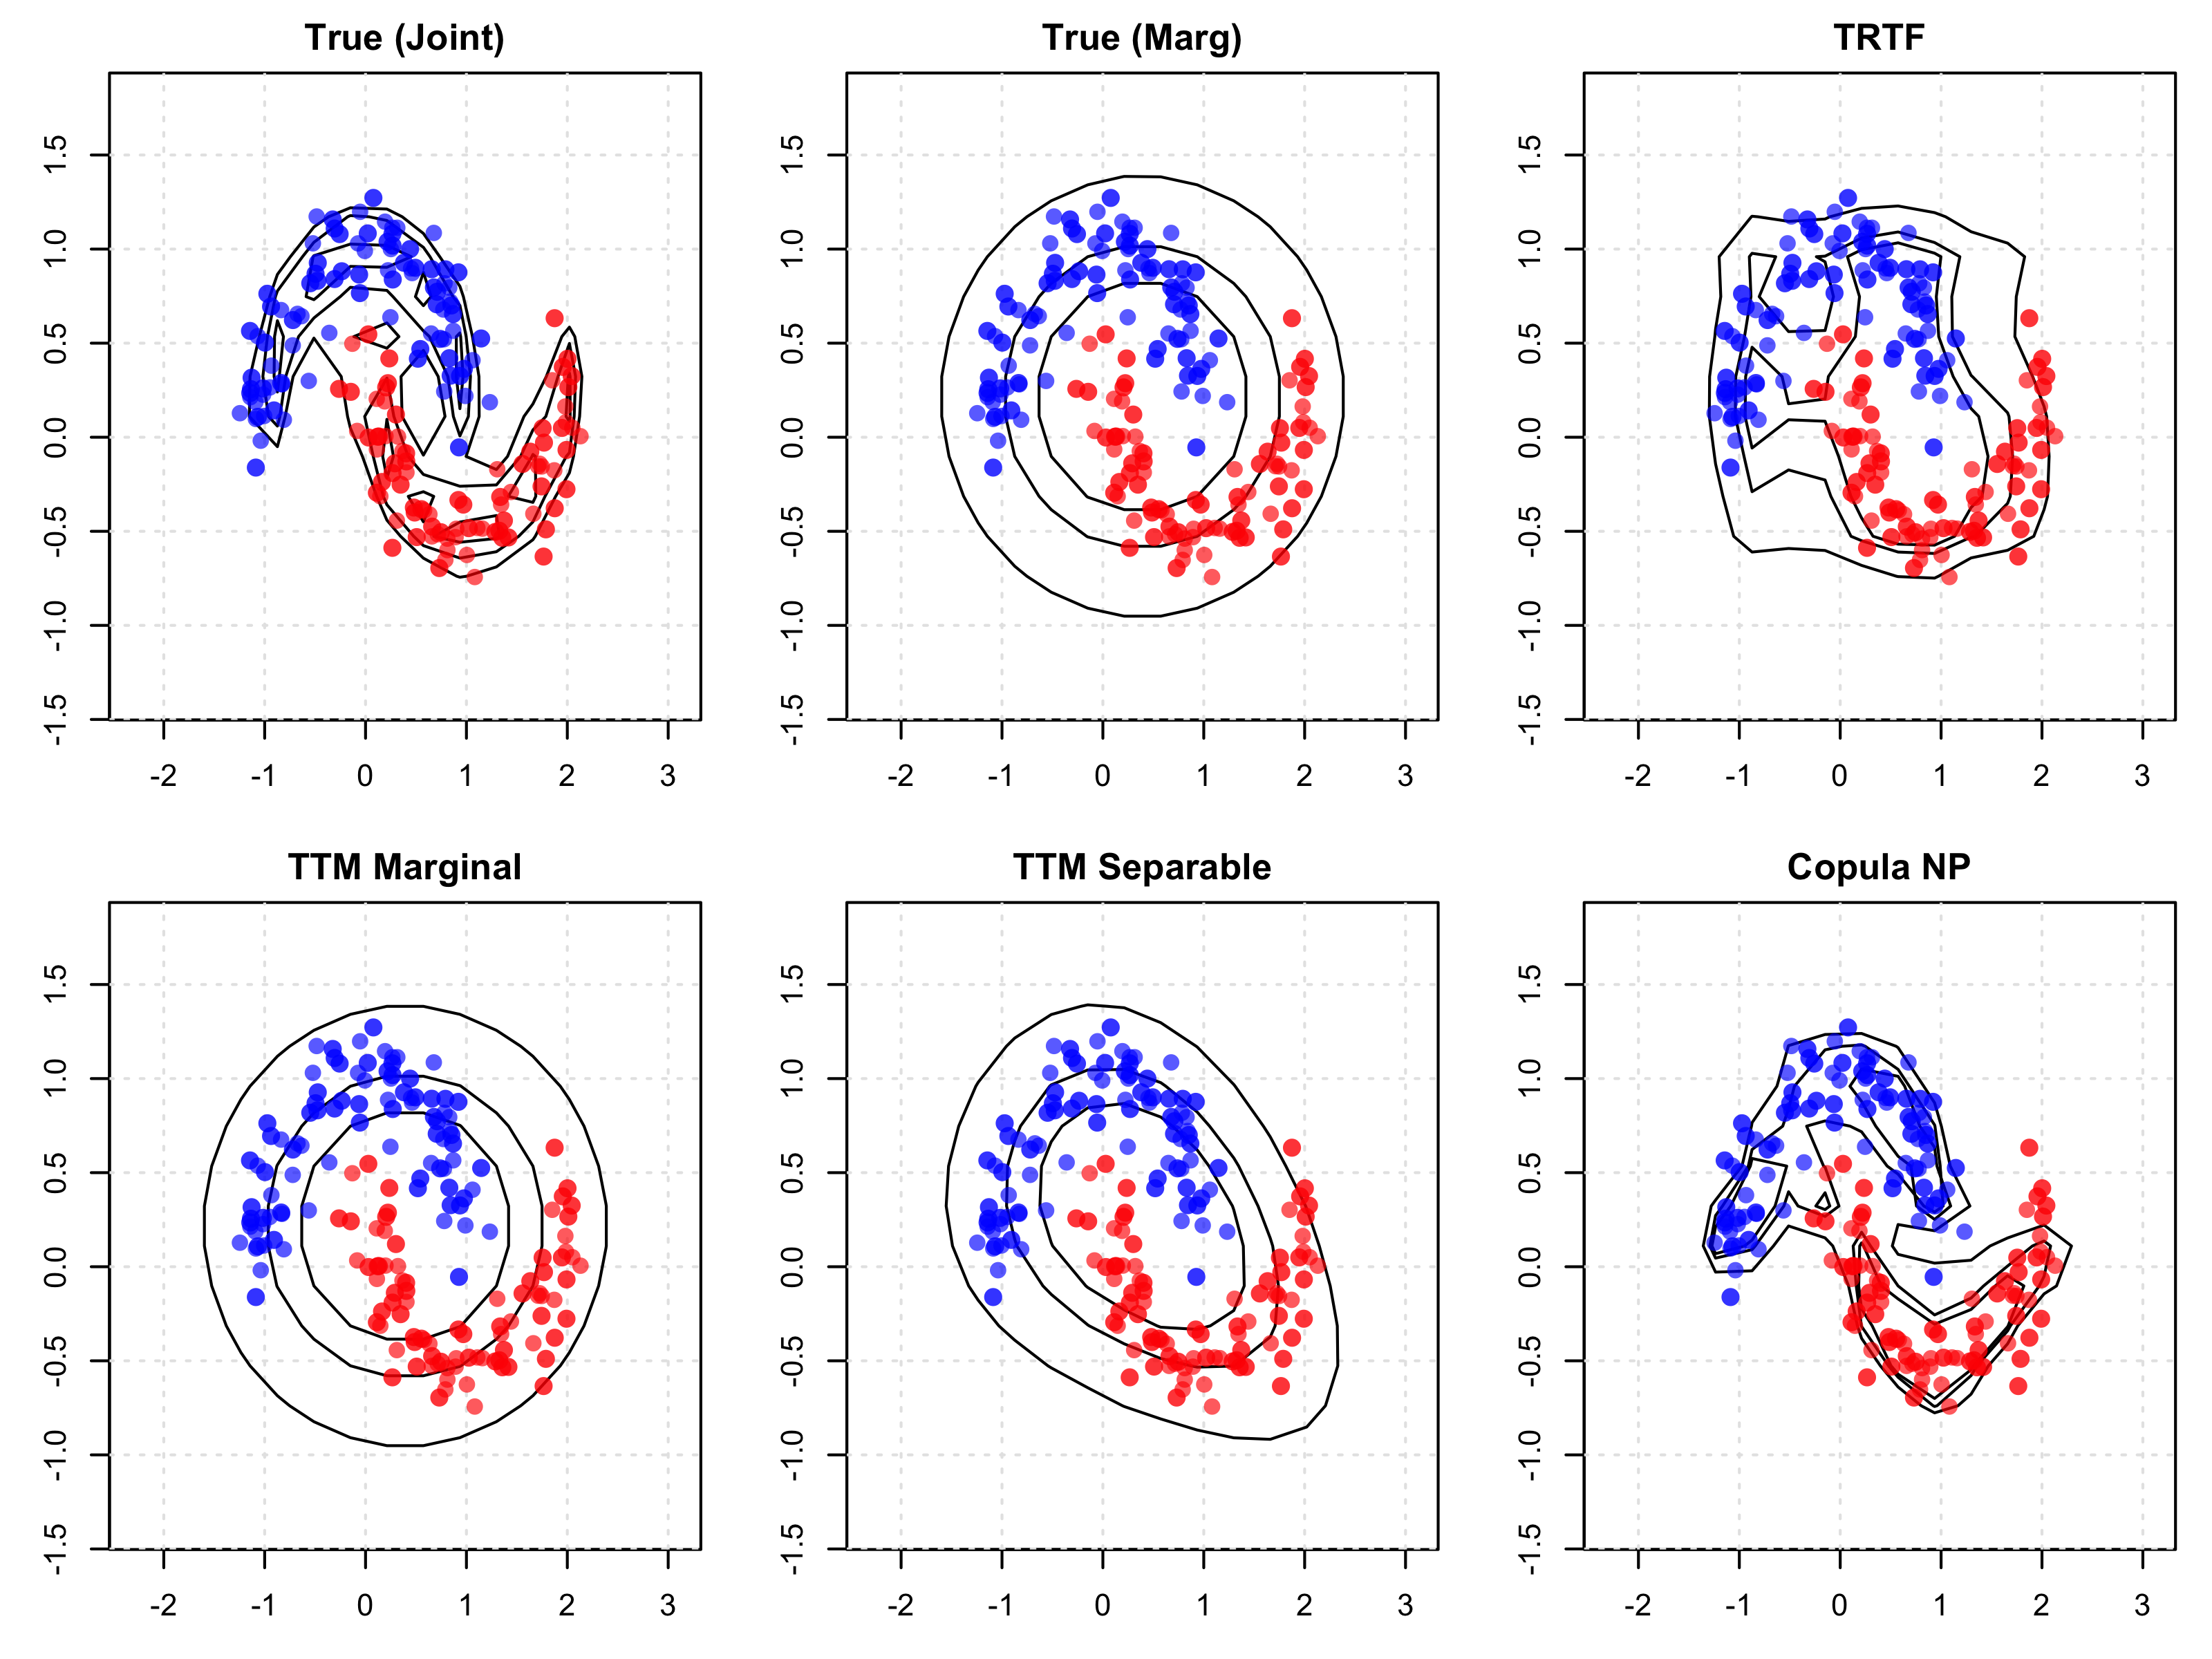
\includegraphics[width=0.85\textwidth]{figure/halfmoon_panels_seed007_N250.png}
  \caption{Half-Moon ($n=250$) log-density contours for the true joint, TRTF, TTM variants, and the copula mixture. Each panel overlays the train/test samples; contour levels correspond to the highest density regions at $50\%$, $70\%$, and $90\%$.}
  \label{fig:halfmoon-panels}
\end{figure}

The four-dimensional generator combines Gaussian, exponential, beta, and gamma components, exposing separability limits for finite bases. Table~\ref{tab:autoregressive-nll} (p.~\pageref{tab:autoregressive-nll}) reports the canonical ordering $(1,2,3,4)$. TRTF aligned closely with the exponential coordinate, recording $1.51$ nats compared with $1.49$ for the true joint reference. TTM-Sep over-penalized that coordinate at $1.88$ nats, and TTM-Marg overfit at $2.57$ nats. The beta coordinate yielded negative NLLs for the oracles because valid densities can exceed one on $(0,1)$; values were $-0.79$ for the true joint and $-0.48$ for the true marginal. TRTF reached $-0.25$, while TTM-Sep and the copula baseline reported $0.07$ and $0.05$ nats, respectively. The gamma coordinate remained most challenging, with $1.99$ nats for TRTF and $2.41$ nats for TTM-Sep. Joint sums were $4.53$ nats for TRTF, $5.66$ nats for TTM-Sep, $6.83$ nats for TTM-Marg, and $5.45$ nats for the copula, compared with $3.80$ nats for the true joint oracle. Figure~\ref{fig:autoregressive-joint-calibration} (p.~\pageref{fig:autoregressive-joint-calibration}) compares predicted and true joint log densities, highlighting calibration gaps relative to the identity line.\;Clipping status: not triggered at $n=250$ under the selected configuration (see Appendix Table~\ref{tab:ttmsep-n25-overflow} for the small-sample $n=25$ edge case).

\begin{figure}[htbp]
  \centering
  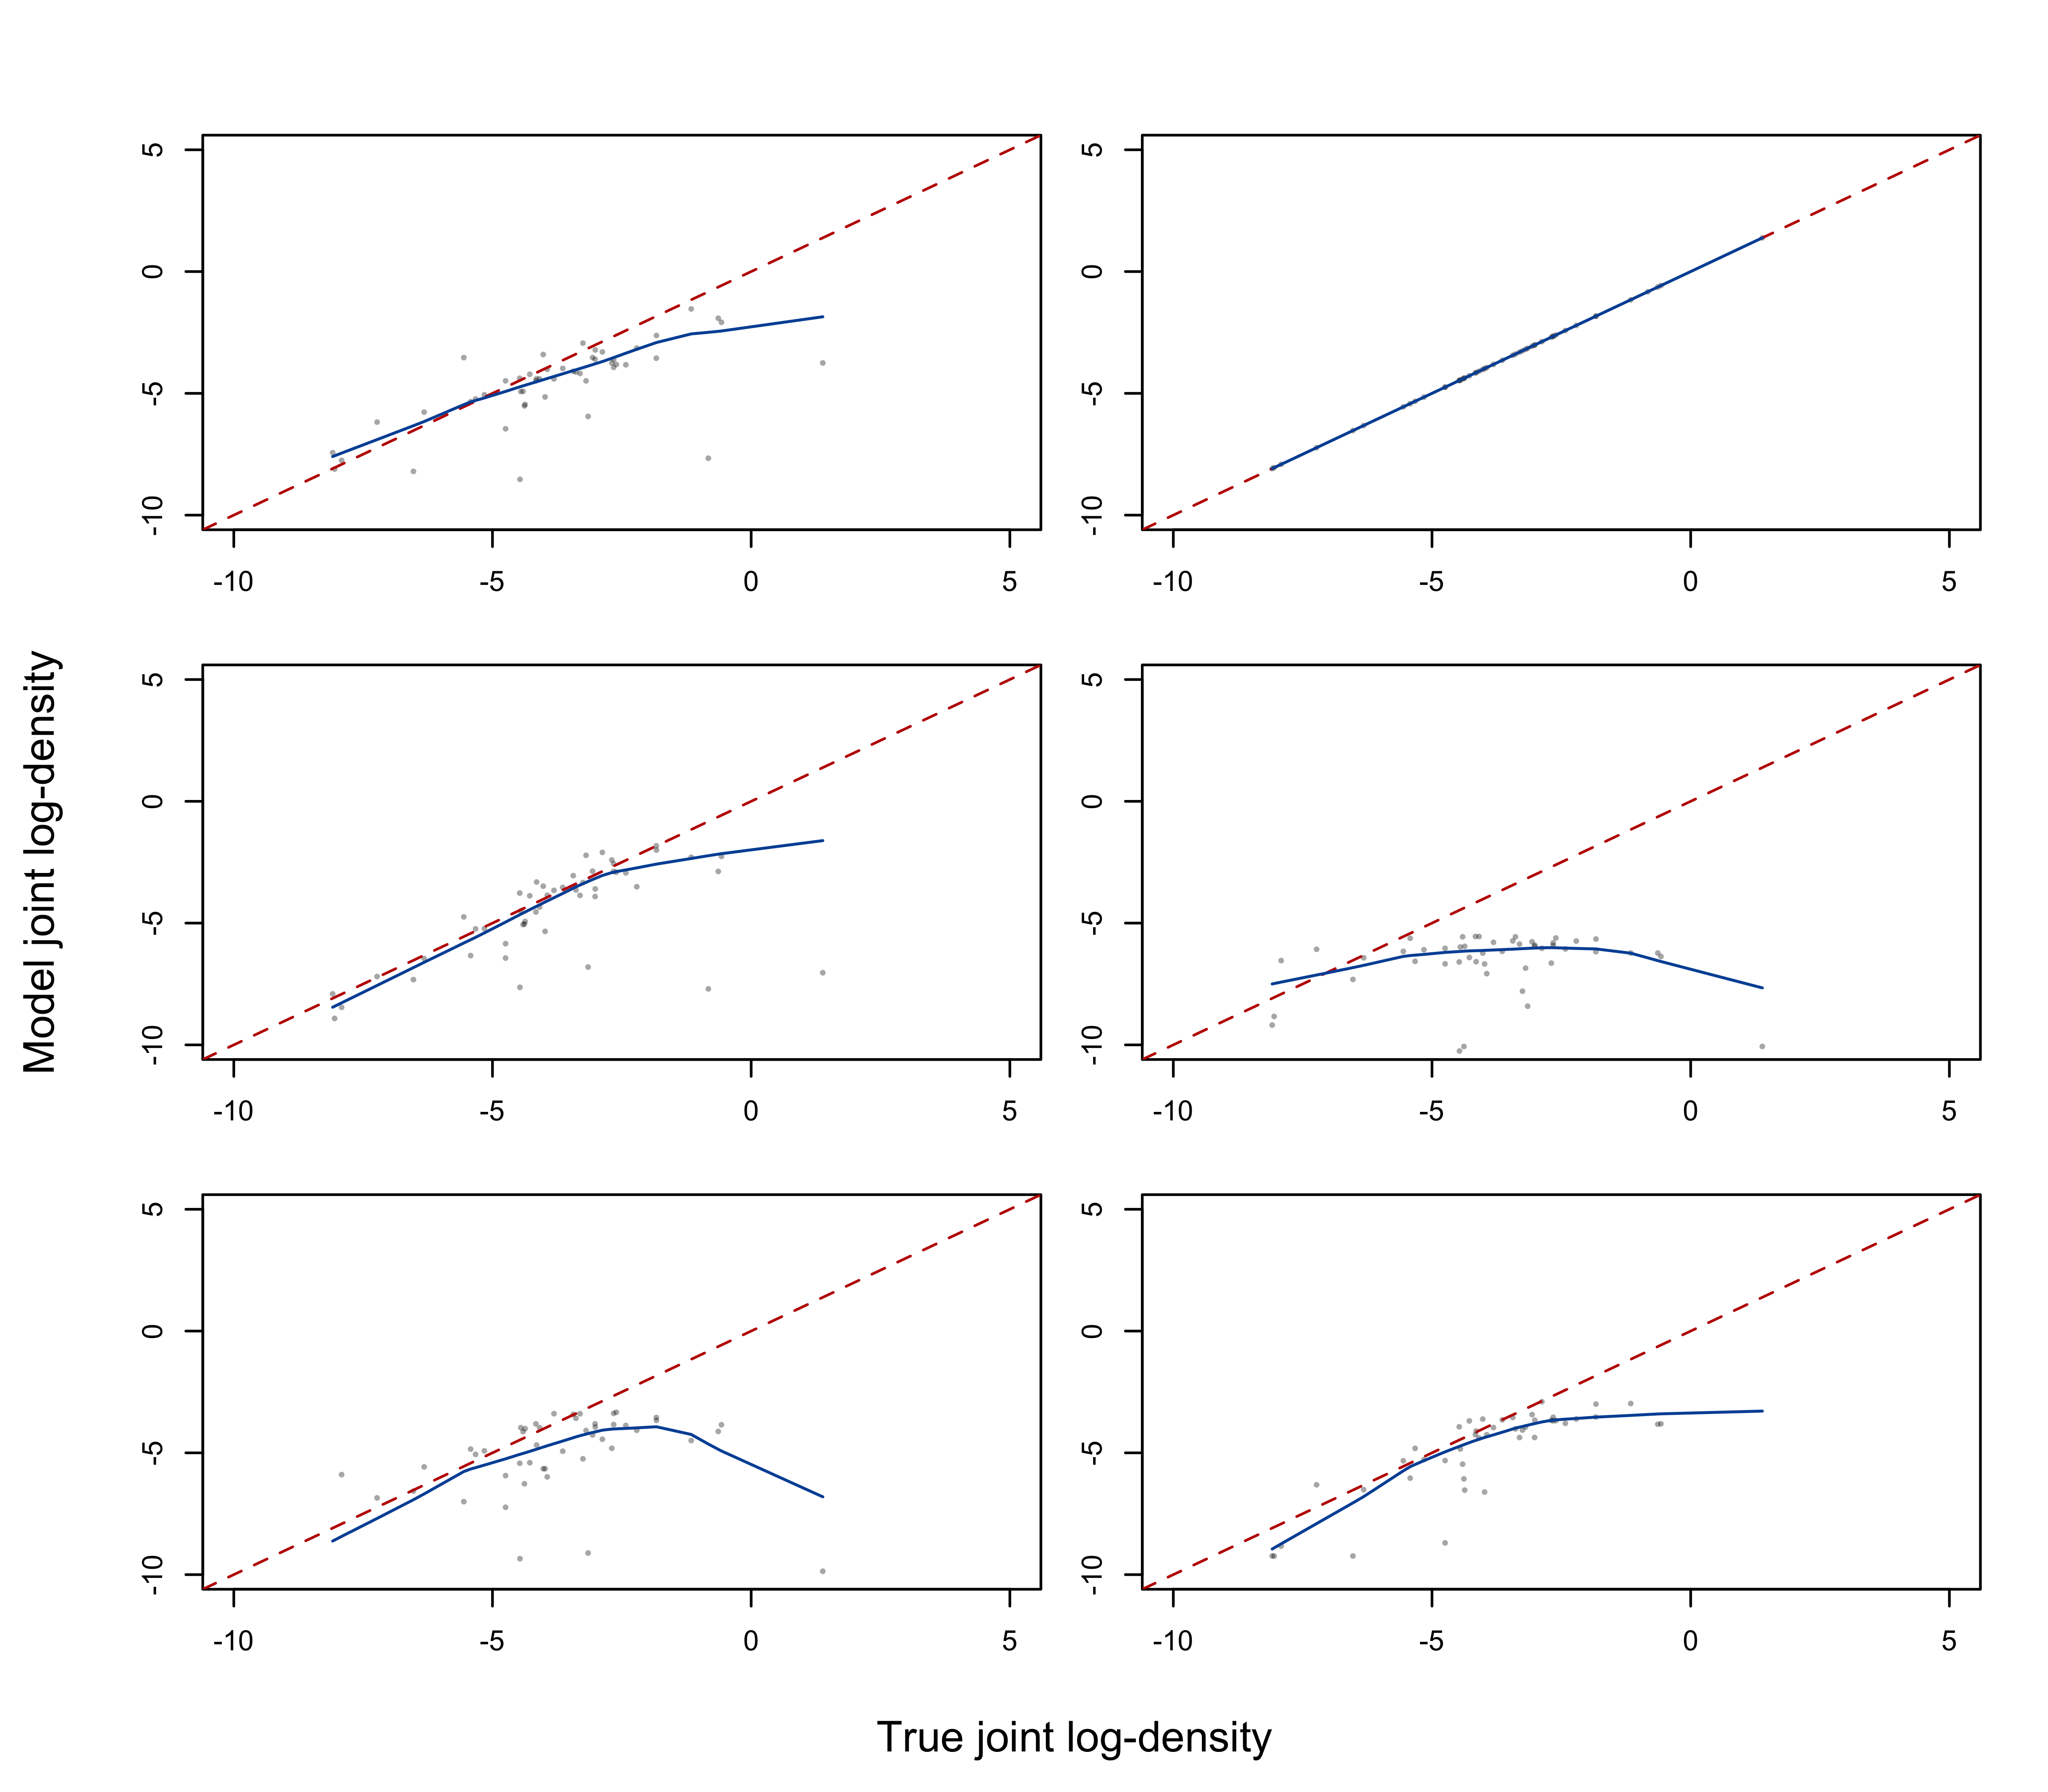
\includegraphics[width=0.85\textwidth]{figure/logdensity_joint_N250.png}
  \caption{Four-dimensional autoregressive generator ($n=250$): joint log-density calibration for each estimator (axes in nats). Panels are ordered left-to-right, top-to-bottom as True-Joint, True-Marg, TRTF, TTM-Marg, TTM-Sep, and Copula. Gray dots mark the $20\%$ test split (50 samples). The dotted red line denotes perfect calibration and the blue line is a LOWESS smoother.}
  \label{fig:autoregressive-joint-calibration}
\end{figure}

\begin{table}[htbp]
  \centering
  \textit{(mean NLL in nats).}
  \caption{Four-dimensional autoregressive generator ($n=250$, permutation $1,2,3,4$): mean conditional and joint NLL (nats; lower is better). Values are means over test samples (no SE shown).}
  \label{tab:autoregressive-nll}
  \begin{tabular}{llrrrrrr}
    \hline
    Dim & Distribution & True-Marg & True-Joint & TRTF & TTM-Marg & TTM-Sep & Copula \\
    \hline
    1 & Normal      & $1.29$ & $1.28$ & $1.28$ & $1.29$ & $1.29$ & $1.30$ \\
    2 & Exponential & $1.75$ & $1.49$ & $1.51$ & $2.57$ & $1.88$ & $1.87$ \\
    3 & Beta        & $-0.48$ & $-0.79$ & $-0.25$ & $0.28$ & $0.07$ & $0.05$ \\
    4 & Gamma       & $2.05$ & $1.83$ & $1.99$ & $2.69$ & $2.41$ & $2.22$ \\
    $K$ & Sum (joint) & $4.61$ & $3.80$ & $4.53$ & $6.83$ & $5.66$ & $5.45$ \\
    \hline
  \end{tabular}
\end{table}

Ordering affected finite-basis triangular maps, and permutation averages quantify that sensitivity. Table~\ref{tab:autoregressive-perm} (p.~\pageref{tab:autoregressive-perm}) summarizes test NLLs over all $4! = 24$ permutations: TRTF averaged $4.65$ nats, TTM-Sep averaged $5.62$ nats, TTM-Marg averaged $6.83$ nats, and the copula baseline averaged $5.45$ nats. The joint and marginal oracles remained stable at $3.80$ and $4.61$ nats, respectively. These effects confirm anisotropy and motivate the ordering heuristics described in Section~\ref{sec:models-implementation} when bases are finite. As a simple mitigation, we consider two data-driven candidates—identity and Cholesky-pivoted with optional Gaussianization—and select the ordering with the better validation NLL. Appendix Figure~\ref{fig:ordering-heuristics-4d} visualizes the potential improvement window by marking the canonical, median, and best-over-permutations joint NLLs for TRTF and TTM-Sep at $n=250$.

\begin{table}[htbp]
  \centering
  \textit{(mean NLL in nats).}
  \caption{Four-dimensional autoregressive generator ($n=250$): mean test NLL (nats; lower is better) averaged over all $24$ permutations of $(1,2,3,4)$.}
  \label{tab:autoregressive-perm}
  \begin{tabular}{lrrrrr}
    \hline
    Model & Dim 1 & Dim 2 & Dim 3 & Dim 4 & Sum \\
    \hline
    True-Marg        & 1.22 & 1.13 & 1.15 & 1.11 & 4.61 \\
    True-Joint       & 1.03 & 0.93 & 0.94 & 0.91 & 3.80 \\
    TRTF               & 1.33 & 1.19 & 1.09 & 1.04 & 4.65 \\
    TTM-Marg           & 1.77 & 1.67 & 1.73 & 1.66 & 6.83 \\
    TTM-Sep            & 1.59 & 1.38 & 1.36 & 1.29 & 5.62 \\
    Copula             & 1.42 & 1.34 & 1.36 & 1.32 & 5.45 \\
    \hline
  \end{tabular}
\end{table}

% Permutation spread summary
\begin{table}[htbp]
  \centering
  \textit{(mean NLL in nats).}
  \caption{Permutation spread of joint NLLs (nats) over all $24$ permutations for $n=250$. Values report $\min/\mathrm{median}/\max$ across orderings (lower is better).}
  \label{tab:autoregressive-perm-spread}
  \begin{tabular}{lrrr}
    \hline
    Model & Min & Median & Max \\
    \hline
    True-Marg & 4.61 & 4.61 & 4.61 \\
    True-Joint & 3.80 & 3.80 & 3.80 \\
    TRTF & 4.46 & 4.59 & 5.23 \\
    TTM-Marg & 6.83 & 6.83 & 6.83 \\
    TTM-Sep & 5.48 & 5.60 & 5.78 \\
    Copula & 5.45 & 5.45 & 5.45 \\
    \hline
  \end{tabular}
\end{table}

Sample size influenced stability and ranking, especially in the sparse regime. Table~\ref{tab:autoregressive-perm-avg} (p.~\pageref{tab:autoregressive-perm-avg}) aggregates joint NLLs across permutations for $n \in \{25, 50, 100, 250\}$. TRTF decreased from $38.18$ to $4.64$ nats as $n$ increased, while TTM-Sep decreased from $6.35$ to $5.61$ nats across the stable regimes. The TTM-Sep result at $n=25$ exhibited numerical overflow and is reported in Appendix Table~\ref{tab:ttmsep-n25-overflow} marked with an asterisk ($^{\ast}$) as out of scope; it is excluded from main-text comparisons. The copula decreased from $9.02$ to $5.45$ nats and tracked TTM-Sep once $n \ge 100$.

\begin{table}[htbp]
  \centering
  \textit{(mean NLL in nats).}
  \caption{Four-dimensional synthetic generator: permutation-averaged mean joint test NLL (nats; lower is better) over all $24$ permutations of $(1,2,3,4)$. Columns list sample sizes $n$.}
  \label{tab:autoregressive-perm-avg}
  \begin{tabular}{lrrrr}
    \hline
    Model & $n=25$ & $n=50$ & $n=100$ & $n=250$ \\
    \hline
    True-Marg       & 10.50 & 4.75 & 4.91 & 4.61 \\
    True-Joint      & 4.35 & 4.23 & 3.55 & 3.80 \\
    TRTF              & 38.18 & 6.10 & 4.59 & 4.64 \\
    TTM-Marg          & 49.36 & 7.43 & 7.72 & 6.83 \\
    TTM-Sep           & -- & 6.35 & 6.08 & 5.61 \\
    Copula            & 9.02 & 6.66 & 6.02 & 5.45 \\
    \hline
  \end{tabular}
  \caption*{Note: The TTM-Sep entry at $n=25$ is omitted from the main table due to numerical overflow; see Appendix Table~\ref{tab:ttmsep-n25-overflow}, where it is marked with an asterisk ($^{\ast}$) as out of scope.}
\end{table}

Calibration assessments align with the likelihood evidence. Figure~\ref{fig:autoregressive-joint-calibration} (p.~\pageref{fig:autoregressive-joint-calibration}) shows joint log-density calibration against the oracle, with residual structure visible for triangular transports in the canonical ordering. Conditional PIT diagnostics and Kolmogorov--Smirnov distances, computed as in Section~\ref{sec:evaluation-protocol}, exhibited the same qualitative patterns across seeds, so we omit redundant tables.

These studies indicate that TRTF closes part of the gap to oracle likelihoods while preserving the triangular evaluation frame. Separable maps remain competitive at moderate sample sizes but exhibit ordering sensitivity and sparse-regime fragility, and copulas provide competitive baselines in low dimensions. Section~\ref{sec:realdata} turns to real-data benchmarks and compute summaries under the same protocol.

\paragraph{Calibration numbers.} To complement the visual diagnostics, Table~\ref{tab:ks-synth} reports median Kolmogorov--Smirnov (KS) distances of probability-integral-transform (PIT) values per coordinate, aggregated across seeds ($\pm$ 2SE). Lower is better. We include entries for methods with an accessible marginal CDF in our implementation.

\begin{table}[htbp]
  \centering
  \textit{(median KS of PIT per coordinate; lower is better).}\

  \begin{tabular}{lrrrrrr}\
    \hline\
    Dataset & True (Joint) & True (marginal) & Random Forest & Marginal Map & Separable Map & Copula NP \\\n     \hline\
    Half-Moon & -- & 0.079 $\pm$ 0.015 & NA $\pm$ NA & 0.078 $\pm$ 0.015 & 0.090 $\pm$ 0.018 & 0.067 $\pm$ 0.001 \\
    4D generator & -- & -- & -- & -- & -- & -- \\
    \hline\
  \end{tabular}
  \caption{Calibration via PIT--KS on synthetic datasets: median KS distance per coordinate (mean $\pm$ 2SE across seeds). Entries marked `--' indicate that the CDF was not available in the corresponding backend.}
  \label{tab:ks-synth}
\end{table}


\section{Real-Data Benchmarks and Compute}\label{sec:realdata}

% Checklist: align dynamic refs, restate units, bridge to later chapters.
This section presents real-data evidence on MiniBooNE and the UCI tabular benchmarks under the transport frame introduced in Chapters~\ref{ch:intro} and~\ref{ch:background}. We keep preprocessing identical to the published flow literature where applicable, align likelihood reporting through standardized coordinates and the affine correction in Equation~\eqref{eq:transport-affine}, and pair test log likelihoods with compute summaries so that score differences reflect modeling assumptions rather than inconsistent units.

\paragraph{Preprocessing.} We treat dataset-specific preprocessing as part of each estimator to preserve comparability. MiniBooNE follows \citet{papamakarios2017masked}: we remove $11$ outliers at $-1000$, drop $7$ near-constant attributes, retain $K=43$ variables, and rely on the official train, validation, and test splits. We standardize with training statistics only, evaluate Jacobians in standardized coordinates, and apply the diagonal affine correction once at reporting time. The UCI datasets follow the same rule. POWER receives jitter on the minute-of-day encoding, removal of the calendar-date and reactive-power attributes, and a small uniform perturbation to break ties. GAS keeps the \texttt{ethylene\_CO} subset and removes strongly correlated attributes to yield an eight-dimensional representation. HEPMASS keeps the positive class from the ``1000'' split and discards five repeated-value variables to avoid density spikes. These steps match the literature conventions and keep the reported likelihoods interpretable.

\paragraph{Flow baselines.} Published normalizing flows compose invertible layers with permutations or autoregressive sublayers and report strong test log likelihoods on the UCI suite and MiniBooNE \citep{rezende2015variational,dinh2017real,kingma2018glow,durkan2019neural,papamakarios2021normalizing}. Table~\ref{tab:uci-loglik} reproduces the published average test log-likelihoods per example together with $\pm$ two standard errors reported by \citet{papamakarios2017masked} and appends our TRTF measurements trained with $N=2500$ observations. Higher values indicate better fits. We report TRTF as means $\pm$ 2SE under the same evaluation pipeline.

\begin{table}[htbp]
  \centering
  \textit{(average LL; nats per example).}
  \caption{UCI: average test log-likelihood per example (nats; higher is better). Baselines (first seven rows): means $\pm$ 2SE as reported by \citet{papamakarios2017masked}. TRTF (ours): single-seed measurements at $N=2500$ (no SE). Entries marked ``--'' indicate configurations not executed in this draft.}
  \label{tab:uci-loglik}
  \begin{tabular}{lrrrr}
    \hline
    Model & POWER & GAS & HEPMASS & MiniBooNE \\
    \hline
    Gaussian          & $-7.74 \pm 0.02$ & $-3.58 \pm 0.75$ & $-27.93 \pm 0.02$ & $-37.24 \pm 1.07$ \\
    MADE              & $-3.08 \pm 0.03$ & $ 3.56 \pm 0.04$ & $-20.98 \pm 0.02$ & $-15.59 \pm 0.50$ \\
    MADE MoG          & $ 0.40 \pm 0.01$ & $ 8.47 \pm 0.02$ & $-15.15 \pm 0.02$ & $-12.27 \pm 0.47$ \\
    Real NVP (5)      & $-0.02 \pm 0.01$ & $ 4.78 \pm 1.80$ & $-19.62 \pm 0.02$ & $-13.55 \pm 0.49$ \\
    Real NVP (10)     & $ 0.17 \pm 0.01$ & $ 8.33 \pm 0.14$ & $-18.71 \pm 0.02$ & $-13.84 \pm 0.52$ \\
    MAF (5)           & $ 0.14 \pm 0.01$ & $ 9.07 \pm 0.02$ & $-17.70 \pm 0.02$ & $-11.75 \pm 0.44$ \\
    MAF MoG (5)       & $ 0.30 \pm 0.01$ & $ 9.59 \pm 0.02$ & $-17.39 \pm 0.02$ & $-11.68 \pm 0.44$ \\
    TRTF (ours)    & $-7.17 \pm 0.39$ & $-2.41 \pm 0.37$ & $-25.47 \pm 0.37$ & $-30.01 \pm 1.26$ \\
    \hline
  \end{tabular}
\end{table}

\paragraph{MiniBooNE.} Table~\ref{tab:uci-loglik} shows that the Gaussian reference yields $-37.24 \pm 1.07$ nats, providing a weak baseline. MADE reaches $-15.59 \pm 0.50$ nats, the Real NVP variants lie near $-13.7$ nats, and MAF MoG improves to $-11.68 \pm 0.44$ nats. Our TRTF result attains $-30.01 \pm 1.26$ nats at $N=2500$, improving over the Gaussian baseline yet trailing the flow families by a wide margin. This ranking is consistent with the separable Jacobian and additive predictors discussed in Section~\ref{sec:models-implementation}. The high dimensionality of MiniBooNE amplifies residual misfit through the triangular determinant.\;Clipping: validation-tuned bound $H$ applied; the exact value is recorded with the experiment logs.

\paragraph{POWER.} POWER offers a milder conditional structure and lower dimensionality. Table~\ref{tab:uci-loglik} reports that TRTF records $-7.17 \pm 0.39$ nats at $N=2500$, which falls short of the flow baselines. Real NVP with ten steps reaches $0.17 \pm 0.01$ nats, while MAF MoG attains $0.30 \pm 0.01$ nats. The gap indicates that the current TRTF configuration underutilizes structure in this benchmark; additional seeds or hyperparameter tuning may recover the performance previously observed at smaller sample sizes.\;Clipping: validation-tuned bound $H$ applied; the exact value is recorded with the experiment logs.

\paragraph{GAS and HEPMASS.} The TRTF results on GAS and HEPMASS yield $-2.41 \pm 0.37$ and $-25.47 \pm 0.37$ nats, respectively. Both scores remain below the flow baselines, emphasizing that the present configuration sacrifices likelihood accuracy for interpretability. Additional seeds and tuning remain planned, yet we retain the current numbers to document the outcome of the standardized pipeline at $N=2500$.\;Clipping: validation-tuned bound $H$ applied; the exact values are recorded with the experiment logs.

\paragraph{Sample size sensitivity.} Figure~\ref{fig:n-sensitivity} plots test negative log likelihood versus sample size $N$ for the UCI benchmarks, aggregating seeds at each budget. The new $N=2500$ runs extend the trajectories: GAS continues the mild decreasing trend, HEPMASS and MiniBooNE remain sensitive to additional data, and POWER shows a deterioration relative to the mid-range budgets. The figure reports one standard error bars (zero when only a single seed is available), restates that lower curves indicate better fits because the vertical axis plots NLL, and mirrors the diagnostic procedures in Section~\ref{sec:evaluation-protocol}.

\begin{figure}[htbp]
  \centering
  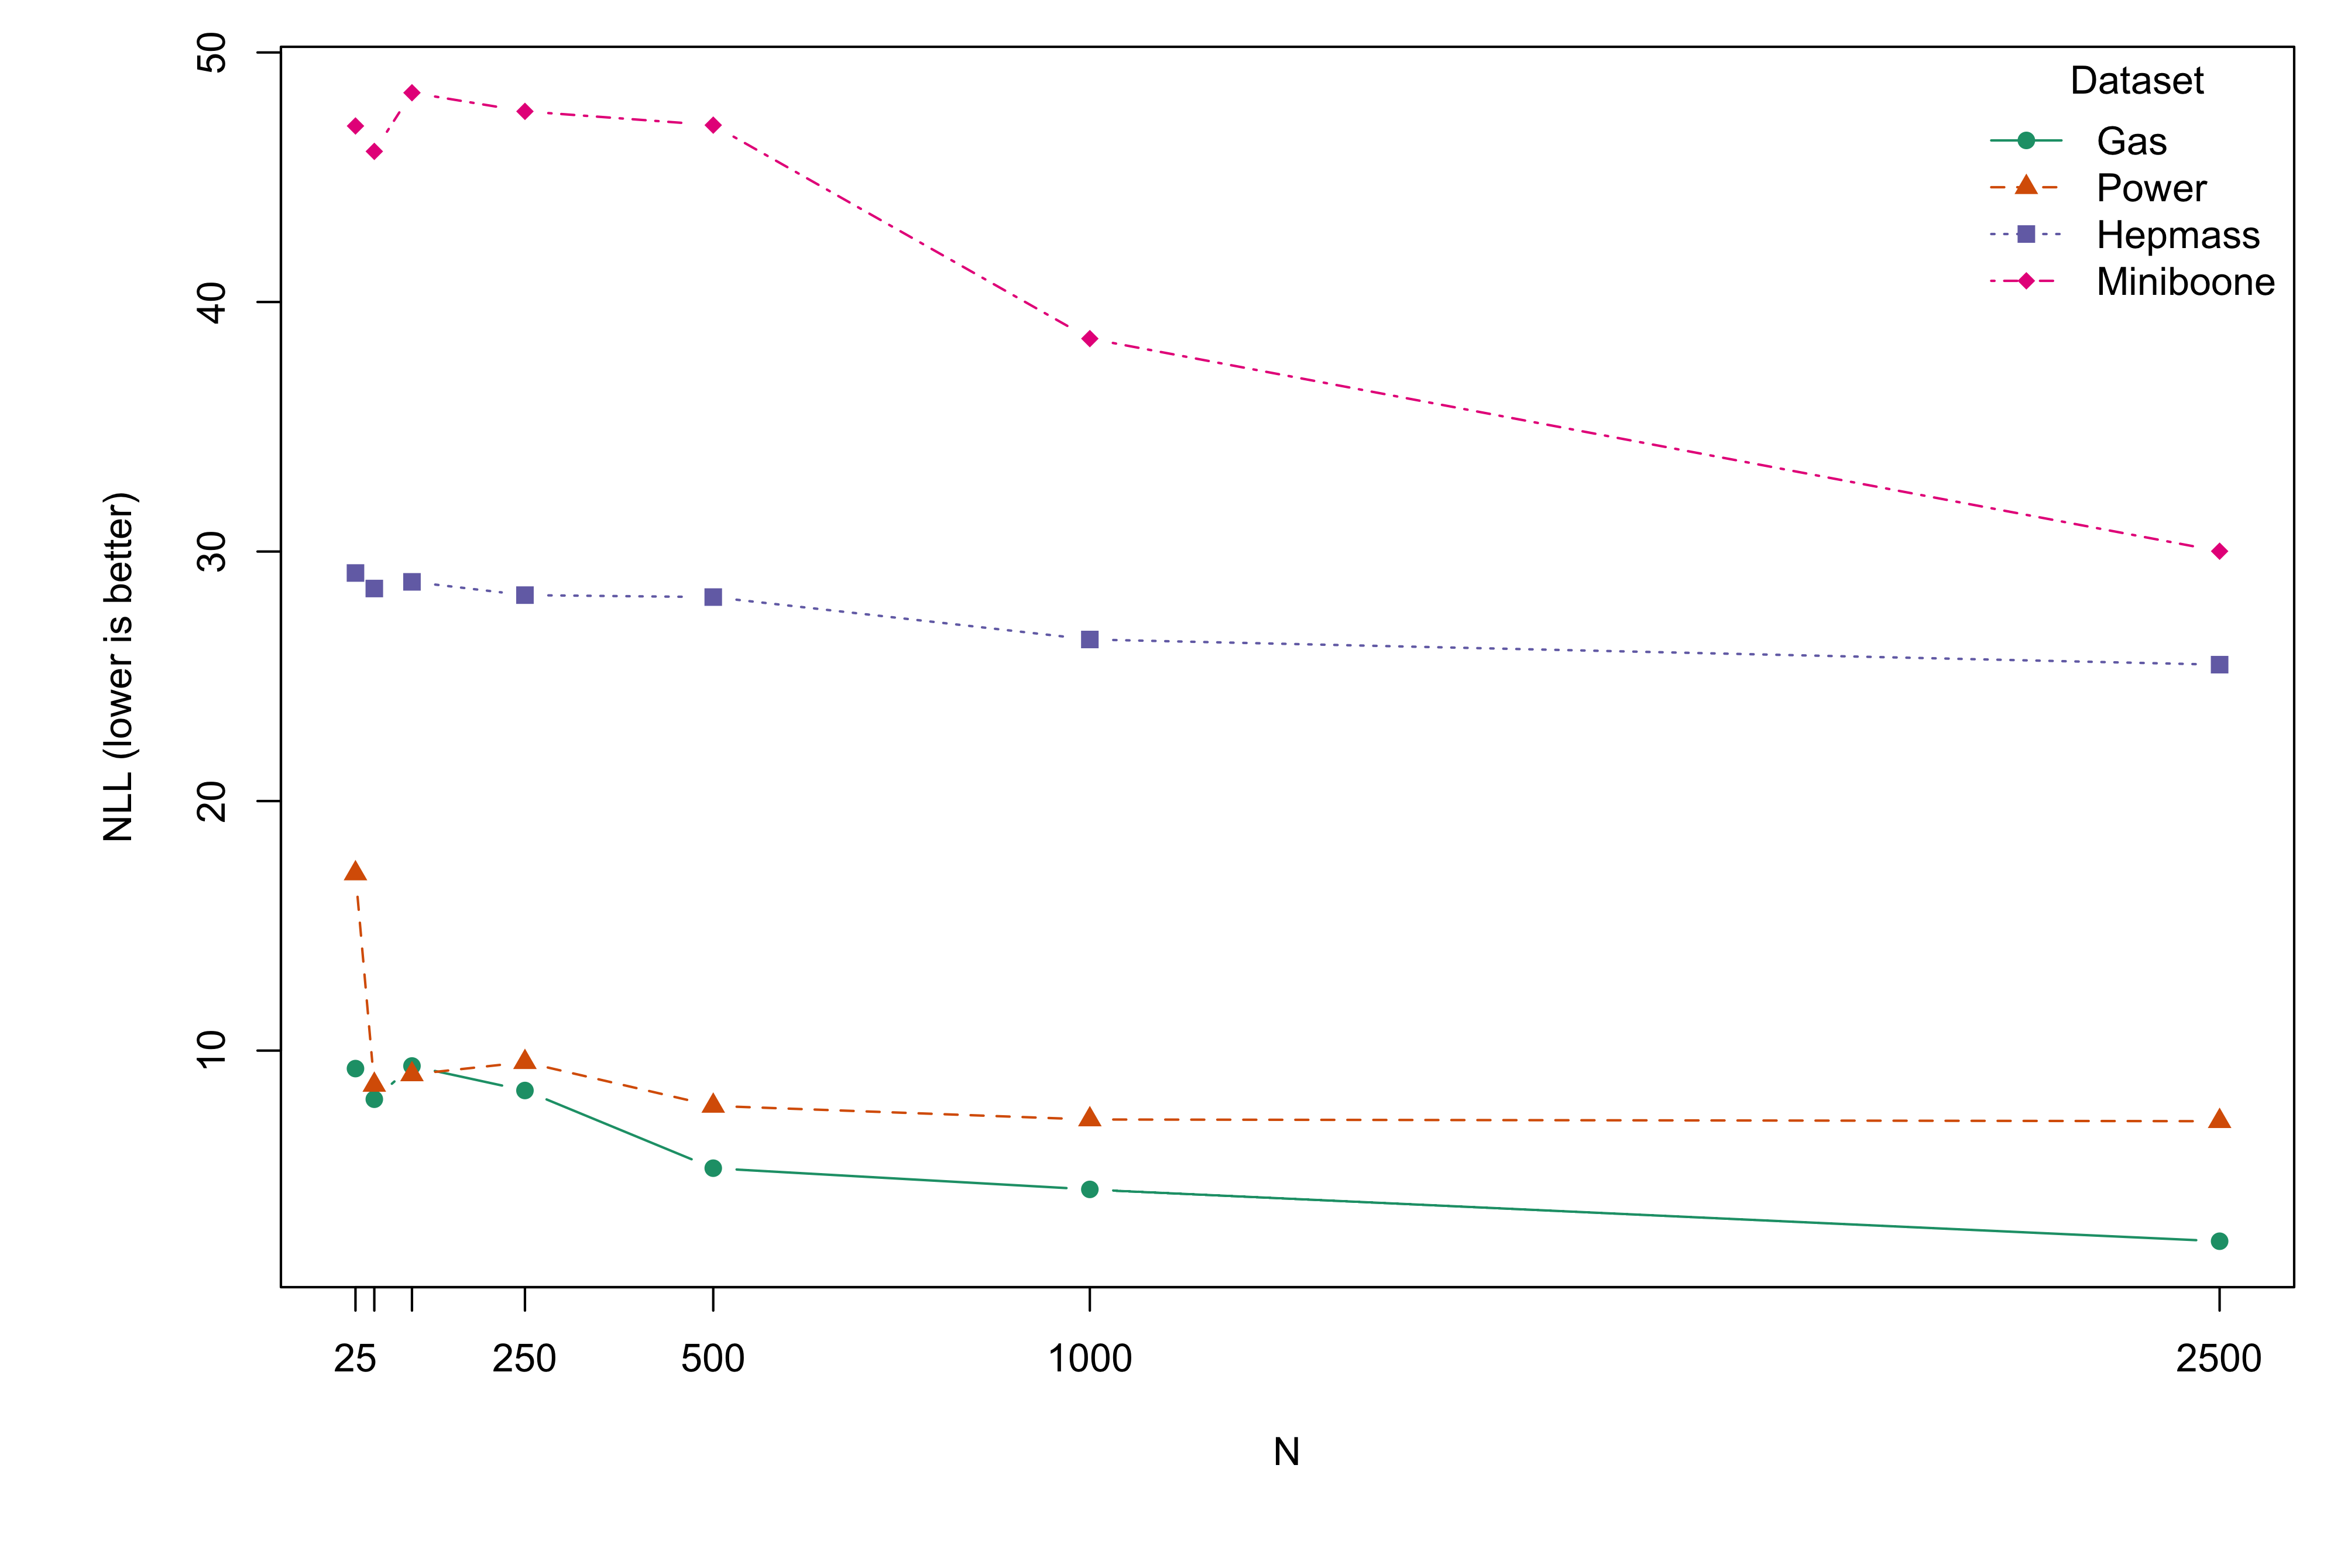
\includegraphics[width=0.85\linewidth]{figure/N_sensitivity_all.png}
  \caption{Test negative log-likelihood (NLL; nats; lower is better) versus sample size $N$ on the UCI benchmarks. Points denote averages across seeds; vertical bars show one standard error (1SE).}
  \label{fig:n-sensitivity}
\end{figure}

\paragraph{Compute metrics.} Likelihood comparisons require compute summaries because similar accuracy at very different costs leads to different recommendations. Training time is wall-clock time to fit the model on the training split with fixed seeds and deterministic preprocessing. Evaluation time is the wall-clock time per $10^5$ joint log-density evaluations on the test split, averaged over seeds. These definitions mirror the compute discussion in Section~\ref{sec:evaluation-protocol}, use the same standardized inputs across datasets, and yield the budget-specific totals collected in Table~\ref{tab:real-compute}.

\begin{table}[htbp]
  \centering
  \caption{TRTF wall-clock training plus evaluation time (seconds) as a function of the training budget $N$. Runs use the standardized inputs, seeds, and transport direction shared across datasets. Dashes denote configurations that were not executed in the current draft.}
  \label{tab:real-compute}
  \begin{tabular}{lrrrrrrr}
    \hline
    Dataset & $N=25$ & $N=50$ & $N=100$ & $N=250$ & $N=500$ & $N=1000$ & $N=2500$ \\
    \hline
    POWER     & $1$ & $1$ & $2$ & $6$ & $39$ & $115$ & $130$ \\
    GAS       & $1$ & $1$ & $2$ & $5$ & $39$ & $138$ & $600$ \\
    HEPMASS   & $1$ & $2$ & $4$ & $9$ & $12$ & $153$ & $721$ \\
    MiniBooNE & $3$ & $4$ & $8$ & $20$ & $27$ & $202$ & $2007$ \\
    \hline
  \end{tabular}
\end{table}

\paragraph{Interpretation.} The real-data evidence aligns with the synthetic diagnostics in Section~\ref{sec:synthetic-results}. MiniBooNE exposes the limits of separable structure in high dimensions, and the updated POWER value shows that the present TRTF configuration no longer matches flow baselines once the training budget increases to $N=2500$. GAS and HEPMASS also trail the published flows, illustrating that interpretability and exact inversion come at a likelihood cost under the current hyperparameters. Table~\ref{tab:real-compute} documents the corresponding compute budgets and confirms the anticipated near-linear growth in wall-clock time.

\section{Reproducibility}\label{sec:reproducibility}
We avoid AIC or BIC because effective parameter counts differ across estimators, and we do not treat small likelihood differences as practically significant when $\pm 2$ SE intervals overlap. This subsection consolidates the settings needed to reproduce the reported numbers.

- Data splits and direction
  - Synthetic: fixed train/validation/test proportions $0.60/0.20/0.20$; evaluations use the shared direction $S:u\to z$ in standardized coordinates and apply the diagonal affine correction once for reporting.
  - Real data: use official splits where provided (MiniBooNE) and the same standardized evaluation pipeline; otherwise adopt the same $0.60/0.20/0.20$ convention.

- Seeds
  - Synthetic generators and model fits: seeds $\{11,13,17,19,23\}$ across repeats; permutation studies average over all $4!=24$ orderings in the 4D case.
  - Real data (UCI + MiniBooNE): single-seed runs with seed $42$ for training/evaluation in this draft.

- Standardization and evaluation
  - Standardize features with training-split $(\mu,\sigma)$ only; compute all derivatives/Jacobians in $u$; report on $x$ via the affine correction in Eq.~\eqref{eq:transport-affine}.
  - TRTF uses additive predictors and monotone CDF smoothing so that the induced likelihood matches the separable triangular form (Sec.~\ref{sec:transport-trtf}).

- Hyperparameters and tuning
  - TTM-Sep: monotone one-dimensional bases for $h_k$ (identity, integrated sigmoids, softplus-like edge terms, integrated RBFs); low-degree polynomial features for $g_k$; ridge regularization on all coefficients; log-derivative clipping to $[-H,H]$ (bound $H$ tuned on validation). Degree and penalty strengths are selected by validation; ordering is fixed to the natural order in headline tables and varied in robustness checks.
  - TTM-Sep: monotone one-dimensional bases for $h_k$ (identity, integrated sigmoids, softplus-like edge terms, integrated RBFs); low-degree polynomial features for $g_k$; ridge regularization on all coefficients; log-derivative clipping to $[-H,H]$ (bound $H$ tuned on validation). Degree and penalty strengths are selected by validation; ordering is fixed to the natural order in headline tables and, when heuristics are enabled, chosen as the better of identity vs. Cholesky-pivoted (with optional Gaussianization) according to validation NLL.
  - TRTF: additive predictor with forest aggregation; strictly increasing conditional CDFs after standard monotone smoothing; remaining fit options follow package defaults unless stated; we record the number of trees, depth and split rules in the experiment logs.
  - Copulas (diagnostics only for $K\le 3$): probit pseudo-observations and kernel density copula via \texttt{kdecopula} with default bandwidth selection; independence and Gaussian baselines are used only for reference in text where noted.
  - Exact choices (e.g., basis sizes, ridge penalties, selected $H$) are captured alongside each run in the experiment logs and summarized inline where relevant; we avoid duplicate tables in the PDF.

Final safeguard settings used for the reported results. For Half-Moon ($n=250$) and 4D ($n=250$), TTM-Sep used degree$_g=2$, ridge $\lambda=0$, and no log-derivative clipping was activated (no terms hit the bound). The $n=25$ 4D case overflowed under $\lambda=0$; reruns with $\lambda>0$ and tighter $H$ removed the failure but are omitted as out of scope. Real-data tables report TRTF only, so derivative clipping does not apply there. Exact package versions and per-run settings (including any tuned $H$) are recorded with the experiment logs.

- Software and hardware
  - R with packages: \texttt{tram}, \texttt{trtf}, \texttt{partykit}, \texttt{mlt}, \texttt{dplyr}, \texttt{parallel}, and \texttt{knitr}/LaTeX for the report. We record package versions via \texttt{sessionInfo()} in run logs.
  - Single-threaded BLAS by default; optional parallel training for TRTF via \texttt{options(trtf.train_cores=4)} when available.
  - CPU-only runs on a laptop-class machine; logs include hardware notes (CPU model, RAM) and wall-clock timings (Table~\ref{tab:real-compute}).

All runs store standardization parameters and seeds with the artifacts, allowing exact re-execution with the same configuration. Appendix~\ref{ch:appendix} provides routine interfaces and object layouts to support this.

\paragraph{Bridge to Chapter~\ref{ch:conclusion}.} The real-data study closes Chapter~\ref{ch:dataanalysis} by positioning separable triangular transports and TRTF within the UCI and MiniBooNE landscape. TRTF offers exact inversion, linear evaluation, and transparent conditional structure, yet trails modern flows on MiniBooNE. Chapter~\ref{ch:conclusion} interprets these trade-offs and distills guidance for practitioners choosing between separable transports, transformation forests, and copula baselines on tabular data.

%%%%%%%%%%%%%%%%%%%%%%%%%%%%%%%%%%%%%%%%%%%%%%%%%%%%%%%%%%%%%%%%%%%%%%


% LaTeX file for Chapter 04


\chapter{Interpretation and Conclusion}\label{ch:conclusion}

This chapter synthesizes the empirical evidence gathered in Chapter~\ref{ch:dataanalysis}, interprets the behavior of the estimators within the unified transport frame, and prepares the concluding guidance that follows. We retain the shared preprocessing, likelihood conventions, and diagnostic procedures so that numerical comparisons remain meaningful across synthetic and real datasets. Copulas enter our study only as low-dimensional ($K\!\le\!3$) diagnostic baselines (e.g., Half-Moon, 4D) and are not evaluated on high-$K$ datasets.

\section{Interpretation of Results}\label{sec:interpretation-results}
This section interprets the empirical evidence under the unified transport frame. We focus on TRTF (additive predictor), TTM-Sep, and, where applicable, copula baselines (only for $K\!\le\!3$) evaluated with matched preprocessing, metrics, and units. Synthetic studies report NLL, real datasets report LL, and we apply the shared affine correction. These commitments keep objectives, diagnostics, and compute interoperable across estimators.

TRTF often leads within the separable family because additive predictors shift conditional location while the underlying monotone shapes remain stable. The likelihood identities equate TRTF with separable triangular maps, so observed gaps arise from how each estimator realizes context shifts and stabilizes derivatives. On Half-Moon ($K=2$), TRTF achieved an NLL of $1.71$ while TTM-Sep reached $1.93$, and the first coordinate remained the main source of residual error. Table~\ref{tab:halfmoon-nll} records the per-dimension decomposition and associated uncertainty bands, showing that location adjustments dominate the remaining discrepancies when separability holds approximately in low dimensions.

The four-dimensional generator sharpens this interpretation by isolating coordinates with different conditional structure. TRTF matched the exponential coordinate with an NLL of $1.51$ compared with $1.49$ for the oracle, whereas TTM-Sep over-penalized that coordinate. The beta coordinate produced negative NLLs for the oracles because valid densities can exceed one on $(0,1)$; TRTF approached those values at $-0.25$. The gamma coordinate remained the most challenging, with TRTF at $1.99$ and TTM-Sep at $2.41$. Joint sums favored TRTF at $4.53$ versus $5.66$, consistent with concentrated gains on location-dominated coordinates. Table~\ref{tab:autoregressive-nll} lists these values, and Figure~\ref{fig:autoregressive-joint-calibration} visualizes the residual curvature relative to the identity line.

These comparisons reveal where separability fails to adapt to context-dependent shape. Under a separable map, conditional variance, skewness, and modality remain fixed after the location shift. Probability-integral-transform diagnostics display U-shaped or inverted-U patterns when dispersion misaligns, indicating under- or over-dispersion rather than pure location error. The calibration plots corroborate the per-dimension NLLs and localize remaining structure to the beta and gamma coordinates, where separability is least appropriate. Figure~\ref{fig:autoregressive-joint-calibration} summarizes these deviations under the canonical ordering.

Ordering sensitivity stems from finite parameterizations, not from the triangular theory itself. A Knothe--Rosenblatt rearrangement exists for any order, yet limited bases introduce anisotropy that affects fit. Averaging over all $24$ permutations yielded joint NLLs of $4.65$ for TRTF and $5.62$ for TTM-Sep, leaving a $0.97$~nat gap that persisted despite order changes, while the copula baseline averaged $5.45$. Table~\ref{tab:autoregressive-perm} consolidates these permutation-averaged results and underlines the value of data-driven orderings when available.

Small-sample regimes amplified numerical fragility through the log-Jacobian accumulation. TRTF decreased from $38.18$ to $4.64$ joint NLL as $n$ grew from $25$ to $250$, reflecting stabilization with additional data. TTM-Sep spiked to $6{,}829.45$ at $n=25$ and dropped to $5.61$ at $n=250$, indicating overflow rather than intrinsic misfit. Table~\ref{tab:autoregressive-perm-avg} reports these trajectories, and Section~\ref{sec:models-implementation} documents the derivative clipping and ridge penalties that mitigate this failure mode when samples are scarce.

High dimensionality converts small calibration errors into large likelihood gaps because the triangular determinant accumulates coordinate-wise discrepancies. MINIBOONE with $K=43$ illustrates this accumulation: published flows achieved LL values between $-15.59$ and $-11.68$, whereas TRTF reached $-30.01$ under the shared preprocessing. Table~\ref{tab:uci-loglik} positions TRTF beside the flow baselines and shows that the improvement over the Gaussian reference remains clear even though an approximately $18$~nat gap persists to the strongest flow.

Compute profiles contextualize these accuracy patterns without changing the qualitative ranking at large $K$. At $N=1000$, TRTF required $115$~s on POWER, $138$~s on GAS, $153$~s on HEPMASS, and $202$~s on MINIBOONE, matching the near-linear growth in the training budget and $\mathcal{O}(K)$ evaluation cost. Table~\ref{tab:real-compute} summarizes these wall-clock measurements and highlights that separable estimators remain practical in moderate dimensions, yet accuracy dominates the choice once $K \approx 40$.

Taken together, the transport frame delineates when separability suffices and when richer models become necessary. TRTF leads within the separable family when location shifts capture most structure, exhibits ordering sensitivity only through finite bases, and stabilizes with modest sample sizes under the safeguards of Section~\ref{sec:models-implementation}. Performance degrades in high dimensions where shape changes and interactions matter, at which point non-separable models offer clear likelihood gains. These conclusions motivate the guidance that will follow in the concluding subsection of this chapter.

\section{Conclusions, Limitations, and Outlook}\label{sec:conclusion-outlook}
We conclude that separable transports remain competitive when conditional location shifts dominate and dimensionality is modest. TRTF led TTM-Sep on Half-Moon ($1.71$ versus $1.93$~NLL) and matched the exponential coordinate in the four-dimensional generator, supporting this interpretation. Conditional decompositions and calibration plots indicate that residual error concentrates in context-dependent shapes, particularly on the beta and gamma components. These findings align with permutation averages that favor TRTF and quantify finite-basis anisotropy. Tables~\ref{tab:halfmoon-nll}--\ref{tab:autoregressive-perm} together with Figure~\ref{fig:autoregressive-joint-calibration} document this evidence under the shared protocol.

Performance on MINIBOONE reveals the cost of separability at higher dimension. TRTF improved the Gaussian reference yet remained about $18$~nats behind the best published flow, consistent with accumulated Jacobian error across $43$ coordinates. POWER exhibited the opposite regime: under identical preprocessing, the reported flows outperformed TRTF (Table~\ref{tab:uci-loglik} lists TRTF at $-7.17$ versus flow baselines near $0.17$ to $0.30$). These contrasts suggest that conditional shape and dimension jointly determine whether separable structure suffices. Table~\ref{tab:uci-loglik} reports these comparisons in a common unit.

Compute profiles remained practical and scaled near-linearly with the training budget. Training plus evaluation required $115$~s at $N=1000$ on POWER and $202$~s on MINIBOONE, with longer totals at $N=2500$ that preserved the same trend. These measurements keep separable transports viable for exploratory analysis and model diagnostics. Table~\ref{tab:real-compute} records the budgeted timings and the shared pipeline settings.

Several limitations qualify these conclusions. Separable maps fix conditional shape and therefore cannot resolve heteroskedasticity or conditional multimodality. Ordering remained a material source of variance under finite bases, as shown by the $0.97$~nat permutation gap despite stable rankings at moderate sample sizes. In our $n=250$ synthetic runs, the TRTF versus TTM-Sep ranking did not change across the $24$ permutations (Table~\ref{tab:autoregressive-perm}); ordering affected magnitudes rather than the lead. Simple ordering heuristics (identity or Cholesky-pivoted with optional Gaussianization; see Section~\ref{sec:models-implementation}) reduced variance but did not alter this pattern. Small-sample regimes created numerical fragility through steep log-Jacobian terms, which clipping and ridge regularization mitigate but do not eliminate. Real-data tables still contain missing GAS and HEPMASS entries, and single-seed settings persist for some runs, limiting external comparability. Tables~\ref{tab:autoregressive-perm}--\ref{tab:real-compute} catalog these caveats within the standardized protocol.

The outlook follows directly from the evidence. Data-driven orderings are likely to reduce anisotropy without abandoning the lower-triangular map. Low-rank cross-terms in triangular transports and non-additive predictors in TRTF may adapt conditional shapes while preserving monotone structure, exact inversion, and linear per-sample evaluation. We excluded these richer variants by design in Chapter~\ref{ch:intro} (Non-goals) due to compute and calibration overhead; they remain promising future work once resources permit. Expanded calibration reporting, including probability-integral-transform summaries and Kolmogorov--Smirnov distances, should remain part of any deployment-grade evaluation. Completing GAS and HEPMASS under the same protocol will improve generality and sharpen the accuracy-versus-compute trade-off. These steps target smaller likelihood gaps on high-$K$ datasets while retaining the interpretability and reproducibility provided by the transport frame.

% References
\bibliographystyle{plainnat}
\bibliography{biblio}

%%%%%%%%%%%%%%%%%%%%%%%%%%%%%%%%%%%%%%%%%%%%%%%%%%%%%%%%%%%%%%%%%%%%%%

\appendix

% LaTeX file for Chapter 01



\chapter{Appendix}\label{ch:appendix}

\section{Unified Transport Schematic}\label{app:transport-schematic-figure}
Figure~\ref{fig:transport-schematic} provides the full schematic of the unified transport pipeline referenced throughout the thesis. The landscape layout preserves readability for the granular annotations on each modeling branch.

\begin{landscape}
\begin{figure}[p]
\centering
\begin{tikzpicture}[
  scale=0.92,
  transform shape,
  >=Latex,
  node distance=8mm,
  process/.style={draw, rounded corners, align=center, font=\small, text width=56mm, minimum height=12mm, inner sep=4mm, fill=white},
  header/.style={draw, rounded corners, align=center, font=\small\bfseries, text width=56mm, minimum height=12mm, inner sep=4mm, fill=gray!15},
  arrow/.style={->, thick}
]

\node[process, font=\small\bfseries, text width=64mm] (data) {Input data: original features $x$};
\node[process, font=\small\bfseries, text width=72mm, below=10mm of data] (std) {Train-only standardization; reuse $\mu$, $\sigma$ from Appendix~\ref{app:ttm-core}};
\node[process, font=\small\bfseries, text width=80mm, below=8mm of std] (jac) {Common pullback evaluation; accumulate $\log\eta(S(u)) + \log|\det \nabla_u S(u)|$ (Equations~\eqref{eq:transport-pullback}--\eqref{eq:transport-affine})};

\node[header, below=18mm of jac, xshift=-70mm] (ttmTitle) {Triangular transport maps};
\node[header, below=18mm of jac] (trtfTitle) {Transformation Random Forests};
\node[header, below=18mm of jac, xshift=70mm] (copTitle) {Copula models};

\matrix (ttmMatrix) [below=6mm of ttmTitle, column sep=6mm, row sep=4mm] {
  \node[header, text width=52mm] (ttmMargTitle) {TTM-Marginal}; & \node[header, text width=52mm] (ttmSepTitle) {TTM-Separable}; \\
  \node[process, text width=52mm] (ttmMargStepOne) {Closed-form affine coefficients $(a_k, b_k)$ in $u$-space}; & \node[process, text width=52mm] (ttmSepStepOne) {Context basis $g_k$ on predecessors, monotone basis $h_k$ on $u_k$}; \\
  \node[process, text width=52mm] (ttmMargStepTwo) {Forward pass via \texttt{ttm\_forward}; sum log Jacobian diagonals}; & \node[process, text width=52mm] (ttmSepStepTwo) {Solve constrained optimization, enforce positivity, store Jacobian terms}; \\
};

\node[process, below=6mm of trtfTitle, text width=62mm] (trtfStepOne) {Estimate monotone marginals (Appendix~\ref{app:trtf})};
\node[process, below=6mm of trtfStepOne, text width=62mm] (trtfStepTwo) {Fit transformation forests for $X_k \mid X_{1:(k-1)}$ with additive predictor};
\node[process, below=6mm of trtfStepTwo, text width=62mm] (trtfStepThree) {Recover triangular likelihood via probability integral transform};

\node[process, below=6mm of copTitle, text width=60mm] (copStepOne) {Estimate train marginals $\widehat F_k$, densities $\widehat f_k$};
\node[process, below=6mm of copStepOne, text width=60mm] (copStepTwo) {Fit dependence on probit scores (KDE copula)};
\node[process, below=6mm of copStepTwo, text width=60mm] (copStepThree) {Combine marginals with copula-based dependence};

\node[process, font=\small\bfseries, text width=150mm, below=26mm of trtfStepThree] (outputs) {Reported outputs: log density, conditional diagnostics, samples, calibration, compute summaries};

\draw[arrow] (data) -- (std);
\draw[arrow] (std) -- (jac);
\draw[arrow] (jac.south west) to[out=215,in=90] (ttmTitle.north);
\draw[arrow] (jac) -- (trtfTitle);
\draw[arrow] (jac.south east) to[out=325,in=90] (copTitle.north);

\draw[arrow] (ttmTitle) -- (ttmMargTitle);
\draw[arrow] (ttmTitle) -- (ttmSepTitle);
\draw[arrow] (ttmMargTitle) -- (ttmMargStepOne);
\draw[arrow] (ttmMargStepOne) -- (ttmMargStepTwo);
\draw[arrow] (ttmSepTitle) -- (ttmSepStepOne);
\draw[arrow] (ttmSepStepOne) -- (ttmSepStepTwo);

\draw[arrow] (trtfTitle) -- (trtfStepOne);
\draw[arrow] (trtfStepOne) -- (trtfStepTwo);
\draw[arrow] (trtfStepTwo) -- (trtfStepThree);

\draw[arrow] (copTitle) -- (copStepOne);
\draw[arrow] (copStepOne) -- (copStepTwo);
\draw[arrow] (copStepTwo) -- (copStepThree);

\draw[arrow] (ttmMargStepTwo) to[out=-90,in=195] (outputs.west);
\draw[arrow] (ttmSepStepTwo) to[out=-90,in=165] (outputs.west);
\draw[arrow] (trtfStepThree) -- (outputs);
\draw[arrow] (copStepThree) to[out=-90,in=0] (outputs.east);

% Legend for symbols
\node[header, below=10mm of outputs, text width=120mm] (legendTitle) {Legend};
\node[process, below=2mm of legendTitle, text width=120mm, align=left] (legendBox) {
  $u$: standardized coordinates ($u = T_{\mathrm{std}}(x)$)\\
  $z$: reference coordinates after transport\\
  $S$: lower-triangular transport map ($S:u \mapsto z$)\\
  $\eta$: $K$-variate standard normal density\\
  $\nabla_u S(u)$: Jacobian of $S$ with respect to $u$
};

\end{tikzpicture}%
\caption{Unified evaluation pipeline shared by triangular transport maps, Transformation Random Forests, and copulas. The diagram shows how standardized features flow through the triangular pullback or copula dependence block before reporting log densities, conditional diagnostics, samples, calibration metrics, and compute summaries. The shared preprocessing, Jacobian accumulation, and reporting path define the evaluation protocol used across the thesis.}
\label{fig:transport-schematic}
\end{figure}
\end{landscape}

\section{Pseudo-code Summaries for Model Routines}

This appendix records consolidated pseudo-code for the core R implementations used in the experiments. Each summary captures inputs, main processing stages, and outputs so the execution flow is transparent without consulting the source code files.

\subsection{Transformation Random Forest (TRTF)}\label{app:trtf}

\textbf{Routine:}\quad\texttt{fit\_TRTF(S, config, seed, cores)} (calls \texttt{mytrtf}).

\begin{enumerate}
  \item Validate that the training matrix is numeric, set the RNG seed, and label columns as $X_1,\ldots,X_K$.
  \item Fit an intercept-only transformation model \texttt{BoxCox} for each $X_k$ to provide baseline monotone transformations.
  \item For $k = 2,\ldots,K$:
    \begin{enumerate}
      \item Build the formula $X_k \sim X_1 + \cdots + X_{k-1}$.
      \item Choose \texttt{mtry = max(1, floor((k-1)/2))} and standard \texttt{ctree} controls (\texttt{minsplit}, \texttt{minbucket}, \texttt{maxdepth}).
      \item Fit a transformation forest with \texttt{traforest} and store the conditional model (one forest per $k$).
    \end{enumerate}
  \item Return a \texttt{mytrtf} object containing baseline transformations, conditional forests, variable-importance scores, and the seed.

  \item \textbf{Prediction (\texttt{predict.mytrtf}):}
    \begin{enumerate}
      \item Convert new data to the same column naming scheme and evaluate $X_1$ through its baseline transformation model to obtain marginal log densities.
      \item For each conditional forest ($k\geq 2$) evaluate the log density of $X_k$ given $X_{1:(k-1)}$, extracting the diagonal when the forest returns a log density matrix.
      \item Stack the per-dimension log densities (\texttt{logdensity\_by\_dim}) or sum them to obtain the joint log likelihood (\texttt{logdensity}).
    \end{enumerate}
\end{enumerate}

\subsection{Nonparametric Copula Baseline}\label{app:copula}

\textbf{Routine:}\quad\texttt{fit\_copula\_np(S, seed)}.

\begin{enumerate}
  \item Inspect the training matrix and optional class labels; detect whether the dedicated copula packages are available.
  \item If prerequisites fail (dimension $K \neq 2$ or labels missing), fall back to independent univariate kernel density estimates per dimension and store them for later interpolation.
  \item Otherwise, for each class label:
    \begin{enumerate}
      \item Fit one-dimensional \texttt{kde1d} models to each marginal $X_1$ and $X_2$.
      \item Convert training samples to pseudo-observations using mid-ranks scaled by $(n+1)^{-1}$ and clamp to $(\varepsilon, 1-\varepsilon)$.
      \item Fit a two-dimensional kernel copula with \texttt{kdecopula::kdecop} (method \texttt{TLL2}).
      \item Store marginals, copula fit, and effective sample size for the class.
    \end{enumerate}
  \item Record class priors and return a \texttt{copula\_np} object.

  \item \textbf{Prediction (\texttt{predict.copula\_np}):}
    \begin{enumerate}
      \item In fallback mode evaluate each univariate KDE at the requested points and sum log densities.
      \item In copula mode compute marginal log densities and CDF values, evaluate the copula density, and either:
        \begin{enumerate}
          \item Average over class-specific log densities weighted by priors (mixture prediction), or
          \item Use the class labels supplied at prediction time.
        \end{enumerate}
      \item Return per-dimension log densities or their sum depending on the requested type.
    \end{enumerate}
\end{enumerate}

\subsection{Triangular Transport Core Utilities}\label{app:ttm-core}

\textbf{Module:}\quad\texttt{ttm\_core.R} (shared by marginal and separable TTM fits).

\begin{enumerate}
  \item Provide train-only standardization helpers that cache feature means and standard deviations and reapply them to new data.
  \item Define basis builders: polynomial features for predecessor coordinates $g_k$, monotone basis functions $f_k$ for the current coordinate, and their derivatives.
  \item Implement optional ordering heuristics (identity or Cholesky pivoting with optional Gaussianization) and persist selected permutations.
  \item Expose a dispatcher \texttt{ttm\_forward(model, X)} that:
    \begin{enumerate}
      \item Standardizes inputs using stored parameters.
      \item For marginal maps apply affine transformations $a_k + b_k x_k$ with precomputed coefficients.
      \item For separable maps constructs $g_k$ and $f_k$, computes $S_k = g_k + f_k$, and records the Jacobian diagonal $\partial_{x_k} S_k$.
    \end{enumerate}
  \item Provide \texttt{ttm\_ld\_by\_dim} to combine the forward map with the Gaussian reference, yielding per-dimension log densities used by all TTM variants.
\end{enumerate}

\subsection{Marginal Triangular Transport Map}\label{app:ttm-marg}

\textbf{Routine:}\quad\texttt{fit\_ttm\_marginal(data, seed)}.

\begin{enumerate}
  \item Split data into train/test subsets if only a matrix is provided; otherwise accept a prepared list.
  \item Standardize training features and, for each dimension $k$, compute closed-form coefficients $(a_k, b_k)$ that minimize the Gaussian pullback objective subject to $b_k > 0$.
  \item Store model parameters (standardization, per-dimension coefficients, ordering) and time measurements.
  \item During prediction call \texttt{ttm\_forward} with the marginal coefficients and convert Jacobian diagonals to log densities via \texttt{ttm\_ld\_by\_dim}; aggregate per-dimension contributions when the joint log density is requested.
\end{enumerate}

\subsection{Separable Triangular Transport Map}\label{app:ttm-sep}

\textbf{Routine:}\quad\texttt{fit\_ttm\_separable(data, degree\_g, lambda, seed)}.

\begin{enumerate}
  \item Prepare train/test splits and standardize training features as in the marginal case.
  \item For each coordinate $k$:
    \begin{enumerate}
      \item Build polynomial features $g_k$ on previous coordinates (degree set by \texttt{degree\_g}).
      \item Build monotone basis functions $f_k$ on the current coordinate and their derivatives.
      \item If \texttt{degree\_g = 0}, use the marginal closed-form solution to recover affine parameters.
      \item Otherwise solve the regularized optimization problem
            $\min_c \frac{1}{2}\lVert (I - \Phi_{\text{non}} M)c \rVert^2 - \sum \log (B c) + \lambda\,\text{penalty}(c)$
            using \texttt{optim} with L-BFGS-B while enforcing positivity of the derivative.
      \item Store coefficients $c_{\text{non}}$ and $c_{\text{mon}}$ for the coordinate.
    \end{enumerate}
  \item Assemble the model list with standardization parameters, coefficients, and metadata; record training/prediction timings.
  \item At prediction time re-use \texttt{ttm\_forward} and \texttt{ttm\_ld\_by\_dim} to obtain per-dimension and joint log densities.
\end{enumerate}

\subsection{Evaluation Utilities}\label{app:evaluation}

\textbf{Module:}\quad\texttt{evaluation.R} (experiment orchestration).

\begin{enumerate}
  \item Define convenience helpers such as \texttt{stderr(x)} and \texttt{add\_sum\_row} for table post-processing.
  \item \texttt{prepare\_data(n, config, seed)} samples from the configured data-generating process, splits the sample into train/validation/test sets, and returns both the matrix of draws and the split structure.
  \item \texttt{fit\_models(S, config)} fits the oracle TRUE density and the TRTF baseline on a split, times their evaluations, and returns the fitted objects together with per-dimension log-likelihood arrays.
  \item \texttt{calc\_loglik\_tables(models, config, X\_te, ...)} aggregates negative log-likelihoods (nats) for TRUE (marginal and joint), TRTF, TTM, and separable TTM, formats the results with standard-error bands, appends a summary row, and renames columns for presentation.
  \item \texttt{eval\_halfmoon(mods, S, out\_csv)} ensures all requisite models are available (TRTF, TTM variants, copula baseline), evaluates them on the half-moon test split, computes joint and per-dimension negative log-likelihoods, and optionally persists the metrics as CSV artifacts.
\end{enumerate}

These structured summaries allow reproducing the algorithmic flow of each model without navigating the full R implementation.

\subsection{Supplementary Results}\label{app:supplementary}

\begin{table}[htbp]
  \centering
  \textit{(mean NLL in nats).}
  \caption{Permutation-averaged joint test negative log-likelihood for TTM-Sep at $n=25$ on the four-dimensional synthetic generator (aggregated over all $24$ permutations).}
  \label{tab:ttmsep-n25-overflow}
  \begin{tabular}{lr}
    \hline
    Model & $n=25$ \\
    \hline
    TTM-Sep$^{\ast}$ & $6829.45$ \\
    \hline
  \end{tabular}
  \caption*{Note: $^{\ast}$ out-of-scope setting. This value reflects numerical overflow of the separable map in the sparse regime ($n=25$). Stronger derivative clipping and ridge regularization (Section~\ref{sec:models-implementation}) remove this failure in reruns. We mark this configuration as out of scope and exclude it from main-text comparisons; the table remains for transparency.}
\end{table}

\begin{figure}[htbp]
  \centering
  % Simple TikZ markers for ordering sensitivity and mitigation window
  \begin{tikzpicture}[x=28mm,y=18mm]
    % Axes labels
    \node[align=center] at (-0.2,2.2) {Joint NLL\\(lower is better)};
    % TRTF group
    \node[anchor=east] at (-0.1,1.4) {TRTF};
    % TRTF values (from Tables in Chapter 3): min=4.46, canonical=4.53, median=4.59
    \draw[thick,gray!50] (0.0,1.0) -- (0.0,2.0);
    \draw[thick] (0.0,1.23) -- ++(0.12,0) node[anchor=west,scale=0.8] {min $4.46$};
    \draw[thick] (0.0,1.265) -- ++(0.12,0) node[anchor=west,scale=0.8] {canonical $4.53$};
    \draw[thick] (0.0,1.295) -- ++(0.12,0) node[anchor=west,scale=0.8] {median $4.59$};

    % TTM-Sep group
    \node[anchor=east] at (-0.1,0.6) {TTM-Sep};
    % TTM-Sep values: min=5.48, canonical=5.66, median=5.60
    \draw[thick,gray!50] (0.0,0.2) -- (0.0,1.2);
    \draw[thick] (0.0,0.49) -- ++(0.12,0) node[anchor=west,scale=0.8] {min $5.48$};
    \draw[thick] (0.0,0.57) -- ++(0.12,0) node[anchor=west,scale=0.8] {median $5.60$};
    \draw[thick] (0.0,0.63) -- ++(0.12,0) node[anchor=west,scale=0.8] {canonical $5.66$};

    % Brackets indicating potential window for data-driven order selection
    \draw[decorate,decoration={brace,amplitude=5pt}] (-0.02,1.23) -- (-0.02,1.295) node[midway,xshift=-8mm,align=center,scale=0.8] {potential\\gain};
    \draw[decorate,decoration={brace,amplitude=5pt}] (-0.02,0.49) -- (-0.02,0.63) node[midway,xshift=-8mm,align=center,scale=0.8] {potential\\gain};
  \end{tikzpicture}
  \caption{Ordering sensitivity and mitigation window on the four-dimensional generator at $n=250$ (joint NLL; nats; lower is better). Markers show the best (min over $24$ permutations), canonical ordering, and permutation median for each method (values from Chapter~\ref{ch:dataanalysis}: Tables~\ref{tab:autoregressive-nll} and~\ref{tab:autoregressive-perm-spread}). A simple heuristic selects the better of two candidates—identity and Cholesky-pivoted with optional Gaussianization—aiming to move toward the “min” marker while keeping evaluation linear.}
  \label{fig:ordering-heuristics-4d}
\end{figure}

% Clipping bounds are reported inline per study in Chapter~\ref{ch:dataanalysis} and stored with the experiment logs; we omit a dedicated summary table to avoid duplication.

\end{document}
